% =============================================================================
% PAPER_FLUX_glueball_flat_band_v1_1.tex   --   draft v1.1, June 15, 2026
% v1.1: sigma_5 promoted to EXACT (gate-grade) -- reproduced in exact finite-field
% arithmetic as a residue modulo three independent primes via a weight-blocked
% GF(p) determinant-sector engine (Appendix nativesigma). Title and abstract
% tightened; the version-history author footnote replaced by a clean submission note.
% v1.0 base: certified SU(3) derivation, exact fourth-order band theorem, exact
% real-space sum-of-squares identity, all-rank SU(N>=3) band-shape theorem,
% SU(3) fifth order, the scale-matched ratio, and (v1.1a) a PROVISIONAL internal m6.
% =============================================================================
\documentclass[11pt]{article}
\usepackage{amsmath,amssymb,amsthm}
\usepackage[margin=1.05in]{geometry}
\usepackage{booktabs}
\usepackage{graphicx}
\usepackage{xurl}
\newtheorem{theorem}{Theorem}[section]
\newtheorem{lemma}[theorem]{Lemma}
\newtheorem{proposition}[theorem]{Proposition}
\newtheorem{corollary}[theorem]{Corollary}
\newtheorem{conjecture}[theorem]{Conjecture}
\newtheorem{remark}[theorem]{Remark}
\newtheorem{assumption}[theorem]{Assumption}
\newcommand{\Tr}{\operatorname{Tr}}
\newcommand{\Nt}{\widetilde N}
\newcommand{\ket}[1]{|#1\rangle}
\newcommand{\bra}[1]{\langle #1|}

\title{Gauss-law protection and exact fourth-order lifting of a
$T_1^{+-}$ glueball band in strongly coupled $SU(N\geq3)$ lattice gauge theory\\[2pt]
\large compact localized states, a real-space sum of squares,
and the all-rank band-shape theorem}
\author{Alexander Smith\thanks{Independent Researcher.
Strong-coupling variable $y=\beta/6=1/g_H^4$ throughout. Every displayed
strong-coupling constant, exact enumeration count, and string-tension coefficient
is machine-certified in exact (rational or finite-field) arithmetic; the verification
chain, certificate hashes, and reproduction steps are collected in
Appendix~\ref{app:verification}, and the determinant-sector $\sigma_5$ certificate in
Appendix~\ref{app:nativesigma}.}}
\date{June 15, 2026}

\begin{document}
\maketitle

\begin{abstract}
We determine the one-excitation band structure of strongly coupled $SU(3)$
Hamiltonian lattice gauge theory in $3{+}1$ dimensions in exact rational
arithmetic, and resolve the first order at which the lowest
charge-conjugation-odd band becomes mobile. At second order the lowest
$C$-odd branch is exactly flat over the Brillouin zone. Its flat subspace is
$\ker B(k)^\dagger$, where the signed hopping symbol factors as
$\widetilde N(k)+4I=B(k)B(k)^\dagger$; compact localized states are the
consistently oriented boundaries of elementary cubes, and flatness is the
chain-complex identity $\partial_2\partial_3=0$. All third-order tromino
processes vanish by a bare-link lemma, so the band remains rigid through
$O(y^3)$:
\[
m_-(k,y)=\frac83+y+\frac{11}{306}y^2
-\frac{109151}{249696}y^3+O(y^4).
\]
Using the complete Hermitian 189-record fourth-order real-space kernel, we
show that this protection fails at the next order in a fully controlled way.
For $X_i=1-\cos k_i$ and the cell-gauge flat vector
$\psi=(e^{ik_2}-1,-(e^{ik_1}-1),e^{ik_0}-1)^T$, the projected coefficient
factorizes exactly as
\[
\psi^\dagger[H_4(k)-qI]\psi
=\frac5{12}\sum_iX_i^2
+\frac{17607806155349}{275331901291200}
 \sum_{i<j}X_iX_j,
\]
where $\|\psi\|^2=2\sum_iX_i$ and
\[
q=-\frac{20721577909065127111}{7250590288602460800}.
\]
This momentum-space factorization lifts exactly to a local real-space
sum-of-squares theorem. If $C=\partial_3$ is the oriented cube-boundary map,
$T_i$ translates cube amplitudes, and
$L_i=(T_i-I)^\dagger(T_i-I)$, then
\[
C^\dagger(H_4-qI)C
=\frac{5}{48}\sum_iL_i^2
+\frac{17607806155349}{1101327605164800}
 \sum_{i<j}(\nabla_i\nabla_j)^\dagger(\nabla_i\nabla_j).
\]
Thus the fourth-order mobility is carried by axial three-cube second
differences and planar four-cube checkerboard differences. Positivity proves that $\Gamma$ is the unique global minimum; elementary
cube inequalities prove that $R=(\pi,\pi,\pi)$ is the unique global
maximum. The fourth-order bandwidth is $\Delta W_4\approx0.4806178691$,
with its exact rational value given below. The lift near $\Gamma$ is quadratic but
direction-dependent, so no ordinary effective-mass Hessian exists there;
near $R$ the curvature is isotropic and negative. Thus the Gauss-law band is
exactly immobile through third order and acquires its first nonzero,
parameter-free dispersion at fourth order. Independently, the shared-link
calculus extends to every $SU(N)$ with integer $N\geq3$: in the reduced
normalization fixed by the $SU(3)$ domino,
\[
t_N=\frac{2N(N^2-4)}{(N^2-1)(4N^2-9)(2N^2-1)}>0,
\qquad t_N\sim\frac{1}{4N^3},
\]
and the group-independent incidence kernel gives a universally flat
closed-surface branch at second order. At fourth order the complete $SU(3)$ source chain is recovered from
Stage 0 through the folded des-Cloizeaux Stage 3I and final kernel assembly
Stage 3J. For every integer $N\geq7$, exact walled-Brauer contraction of the
4,171 ordered words gives
\[
D_N(k)=A_N\sum_iX_i^2+B_N\sum_{i<j}X_iX_j,
\quad
q_N=-\frac{2}{3N}\frac{Q_{32}(N^2)}{D_{34}(N^2)},
\]
\[
A_N=\frac{640}{N(N^2-1)^3},
\qquad
B_N=\frac{P_{17}(N^2)}{N R_{20}(N^2)}.
\]
Exact denominator factorizations and positive Newton expansions prove
$q_N<0$, $A_N>0$, and $B_N>0$ in the stable range. A separate exact
$N$-ality scan and determinant-sector contraction then closes the band shape
at the exceptional ranks: the $SU(4)$ determinant contribution satisfies
$\Delta A_4=\Delta B_4=0$, no determinant assignment occurs for $SU(5)$,
and the sole $SU(6)$ determinant orbit is absent from the $A/B$ target.
Together with the rank-specific $SU(3)$ coefficients, this proves a unique
minimum at $\Gamma$, a unique maximum at $R$, and bandwidth $A_N+B_N>0$
for every integer $N\geq3$. The determinant offsets $q_4,q_6$ are given. In pure $SU(2)$ charge conjugation is a
gauge transformation, so the $C$-odd sector is empty and $N\geq3$ is the maximal
domain. Continuing to fifth order in $SU(3)$, the projected coefficient keeps the
identical two-invariant form with $A_5=313/240$ and $B_5>0$, so the
unique-minimum/unique-maximum structure persists through $O(y^5)$. Combined with the
project-native Hamiltonian string tension (bridge $\sigma(y)=\tfrac12W(2y)$) this
gives the scale-matched ratio $m_{1^{+-}}/\sqrt\sigma$ through $O(y^5)$. The
strong-coupling series alone does not reach the continuum---its fourth-order
truncation peaks well below the physical ratio and standard resummations fail---but
the exact $1/N^2$ band structure supplies the functional form for a held-out
extrapolation of continuum lattice data across rank, reproducing the independently
measured large-$N$ value and predicting $m_{1^{+-}}/\sqrt\sigma|_{SU(3)}\approx6.15$
against the measured $6.065(40)$. The $C$-even band and the $T_1^{+-}$
quantum-number assignment are also given exactly. No continuum mass is claimed from
the series itself; the large-$N$ estimate is a lattice-data extrapolation made
trustworthy by the exact $1/N^2$ form.
\end{abstract}

\section{Introduction}
\label{sec:intro}

Flat bands --- single-particle dispersions that are exactly constant over the
Brillouin zone --- arise from destructive interference encoded in lattice
geometry and are spanned by compact localized states (CLS)
\cite{Sutherland1986,Lieb1989,Mielke1991,Tasaki1992,BergmanWuBalents2008,
LeykamAndreanovFlach2018}. They are usually discussed in engineered
condensed-matter, photonic, and cold-atom systems. Here the same structure
appears without geometric engineering in strongly coupled $SU(3)$
Hamiltonian lattice gauge theory \cite{KogutSusskind1975}.

In the strong-coupling regime the elementary one-flux excitations are single
plaquettes of chromoelectric flux. Degenerate perturbation theory turns the
three plaquette orientations into a $3\times3$ Bloch problem. The main
results are:

\begin{itemize}
\item[(A)] At second order the lowest $C$-odd band is exactly flat, with
coefficient $11/306$ at every momentum (Theorem~\ref{thm:flatband}).
\item[(B)] The flat subspace is a lattice Gauss-law kernel. The signed
adjacency factors through the plaquette-boundary incidence map, and the
compact localized states are oriented boundaries of elementary cubes
(Theorems~\ref{thm:gausslaw} and \ref{thm:cls}).
\item[(C)] Every third-order tromino amplitude vanishes by a bare-link
argument. The flat band therefore shifts rigidly by the exact coefficient
$-109151/249696$ (Theorem~\ref{thm:thirdorder}).
\item[(D)] The complete fourth-order kernel breaks the flatness. Its
projection onto the lower-order flat branch factorizes into two positive
cubic invariants in $X_i=1-\cos k_i$ (Theorem~\ref{thm:y4factor}).
\item[(E)] The projected operator has an exact local real-space
sum-of-squares representation. Its two elementary deformations are an axial
three-cube second difference and a planar four-cube checkerboard difference
(Theorem~\ref{thm:y4sos}).
\item[(F)] The factorization gives an analytic global theorem: $\Gamma$ is
the unique band minimum, $R$ the unique band maximum, and the exact
fourth-order bandwidth is $\Delta W_4=A+B$
(Theorem~\ref{thm:y4edges}).
\item[(G)] The rest-point lift is direction-dependent. The $\Gamma$ band
coefficient is continuous and differentiable but has no ordinary Hessian;
the $R$ curvature is isotropic and negative
(Proposition~\ref{prop:y4curvature}).
\item[(H)] The rest-frame $C$-odd triplet transforms as $T_1^{+-}$, while
the $C$-even sector splits as $A_1^{++}\oplus E^{++}$ and disperses normally
(Theorems~\ref{thm:flatband} and \ref{thm:ceven}).
\item[(I)] The signed shared-link hopping is positive for every $SU(N)$,
$N\geq3$, with exact rational coefficient $t_N$ and large-$N$ behavior
$t_N\sim1/(4N^3)$. Since the incidence kernel is group-independent, the
closed-surface second-order branch is universally flat
(Theorem~\ref{thm:suniversal}).
\item[(J)] At fourth order, the full stable-rank contraction is closed for
every integer $N\geq7$. Exact walled-Brauer trace wiring gives $q_N$,
$A_N=640/[N(N^2-1)^3]$, and the canonical compact form
$B_N=P_{17}(N^2)/[N R_{20}(N^2)]$; exact Newton-positivity certificates prove
$q_N<0$, $A_N>0$, and $B_N>0$ (Theorem~\ref{thm:sunfull}).
\item[(K)] Exact determinant-sector reductions extend the band-shape result
to every integer $N\geq3$: $SU(4)$ contributes zero to both invariants,
$SU(5)$ has no determinant assignments, and the sole $SU(6)$ determinant
orbit misses the $A/B$ target. Hence $\Gamma$ and $R$ are the unique global
edges and $A_N+B_N>0$ for all non-pseudoreal ranks
(Theorem~\ref{thm:sunallband}).
\end{itemize}

The physical statement is therefore finite-order and sharp. A closed-surface
$T_1^{+-}$ excitation cannot propagate through the link-mediated channels
that occur through $O(y^3)$: every boundary-link amplitude cancels exactly.
At $O(y^4)$, site-mediated geometries activate and the cancellation no longer
protects the projected branch. The resulting mobility is not inferred from a
scan; it is fixed by an exact positive rational factorization.

The second-order calculation also corrects the $C$-even nearest-neighbor hop
quoted in the companion manuscript \cite{companion}. The missing
vacuum-mediated route changes it to
$t_+=-481/612+3/4=-11/306$, independently adjudicated by exact
two-plaquette diagonalization. The corresponding per-bond ratio
$|t_-|/|t_+|=5/22$ does not itself explain immobility; the incidence kernel
does.

Strong-coupling expansions of Hamiltonian lattice gauge theory have a long
history \cite{KogutSusskind1975,Banksetal1977,KogutSinclairSusskind1976,
Creutz1983}, and the continuum glueball spectrum is accurately known from
Euclidean Monte Carlo \cite{MorningstarPeardon1999,AthenodorouTeper2020}.
The present statements are exact order-by-order results in the
strong-coupling Hamiltonian expansion. They do not predict a continuum mass,
do not establish convergence of the series, and do not claim all-orders
flatness.

Section~\ref{sec:setting} fixes conventions. Sections~\ref{sec:towers} and
\ref{sec:leakage} derive the one-plaquette and shared-link constants.
Section~\ref{sec:band} proves the second-order band structure and compact
localized states. Section~\ref{sec:thirdorder} proves third-order rigidity.
Section~\ref{sec:robust} gives the link-channel robustness theorem, solves the
$SU(3)$ fourth-order band analytically, derives its exact real-space SOS
operator, and proves the complete stable-rank
$SU(N\geq7)$ fourth-order band theorem. Section~\ref{sec:numbers}
summarizes the exact data and physical consequences; Section~\ref{sec:outlook}
lists the remaining problems.

\section{Setting}
\label{sec:setting}

We work with the Kogut--Susskind Hamiltonian \cite{KogutSusskind1975} for
$SU(3)$ on a cubic spatial lattice ($d=3$),
\begin{equation}
H_\beta \;=\; \frac12\sum_{\ell} C_2(\ell)\;+\;\beta\sum_{p}
\Bigl(1-\tfrac1N\,\mathrm{Re}\,\Tr U_p\Bigr),\qquad N=3,
\label{eq:H}
\end{equation}
in units of the electric coupling; $C_2(\ell)$ is the quadratic Casimir on
link $\ell$ and $U_p$ the oriented plaquette holonomy. We use the natural
strong-coupling variable
\begin{equation}
y \;=\; \tfrac{\beta}{6}=\tfrac{1}{g_H^4}, \qquad \beta=6y,
\end{equation}
in which the one-plaquette energy scale is $8/3$ and the perturbation per
plaquette carries one power of $y$. The strong-coupling vacuum is the
electric ground state $\ket{0}$ (all links in the trivial representation);
the elementary excitations are single-plaquette flux states. With
$\chi_p=\Tr U_p$ the fundamental character on plaquette $p$, the normalized
one-flux states of definite charge conjugation are
\begin{equation}
\ket{p,\pm}=\frac{\chi_p\pm\bar\chi_p}{\sqrt2}\,\ket{0},
\qquad C\ket{p,\pm}=\pm\ket{p,\pm},
\end{equation}
with unperturbed energy $8/3$ (four links in the fundamental representation:
$4\times\tfrac12\cdot\tfrac43=\tfrac83$; we keep the conventions of
\cite{companion} throughout). On the cubic lattice plaquettes carry three
orientations $(\mu\nu)\in\{xy,yz,zx\}$, so each momentum sector is a
$3\times3$ problem.

Degenerate strong-coupling perturbation theory in the one-flux manifold
produces, order by order in $y$, an effective hopping Hamiltonian
$H_{\mathrm{eff}}(k)$ per charge sector. Two structural facts organize the
computation: (i) within-plaquette processes renormalize the diagonal and are
captured exactly by the one-plaquette towers of Section~\ref{sec:towers};
(ii) the leading inter-plaquette processes are mediated by \emph{shared
links} --- each plaquette has exactly $4(2d-3)=12$ shared-link neighbors in
$d=3$ (four coplanar, eight transverse) --- and reduce to balanced Haar
moments on the shared link \cite{companion}. We use the linked-cluster
bookkeeping of \cite{companion} (its Assumption~6.5); all finite-system
counting is verified non-perturbatively by exact diagonalization on the
two-plaquette ``domino'' (Section~\ref{sec:leakage}).

\section{One-plaquette towers and the bridge}
\label{sec:towers}

The $SU(3)$ one-plaquette class Hamiltonian
$h_\beta=\tfrac12 C_2+\beta(1-\tfrac13\mathrm{Re}\Tr g)$ restricted to class
functions has charge-even and charge-odd gaps $\Delta_\pm(\beta)$ with exact
strong-coupling towers \cite{companion}
\begin{equation}
\Delta_\pm(\beta)=\tfrac23 \mp \tfrac{\beta}{6}
+ b_2^\pm\beta^2 + b_3^\pm\beta^3 + O(\beta^4),
\qquad
b_2^+=\tfrac{13}{180},\; b_3^+=\tfrac{101}{2700},\;
b_2^-=\tfrac{1}{18},\; b_3^-=\tfrac{7}{432}.
\end{equation}
The bridge to the lattice one-flux sector evaluates the one-plaquette gap at the
local class coupling $b=\beta/4=3y/2$ (one quarter of the lattice coupling), with
an overall factor $4$: the \emph{within-plaquette} part of
the effective one-flux energy is $4\Delta_\pm(3y/2)=4\Delta_\pm(\beta/4)$, i.e.
\begin{equation}
\underbrace{\tfrac83 \mp y + \tfrac{13}{20}y^2 + \tfrac{101}{200}y^3}_{C\text{-even}},
\qquad
\underbrace{\tfrac83 + y + \tfrac12 y^2 + \tfrac{7}{32}y^3}_{C\text{-odd}},
\label{eq:towers}
\end{equation}
to the orders needed here. Everything beyond \eqref{eq:towers} is
inter-plaquette leakage, computed in the next two sections.

\section{Second order: exact leakage and the corrected $C$-even hop}
\label{sec:leakage}

At $O(y^2)$ the only inter-plaquette geometry is the shared-link pair.
Integrating the six free links of the pair by the fusion identity
$\int dB\,\Tr(XB)\Tr(YB^\dagger)=\Tr(XY^\dagger)/3$ reduces every required
quantity to balanced $(2,2)$ Haar moments on the shared link, resolved into
the irreducible channels $\{1,8,\bar3,6\}$ of the fused link representation,
with dimension-weighted norms $N_R=d_R/9$. The corresponding intermediate
energies are $\{4,\tfrac{11}{2},\tfrac{14}{3},\tfrac{17}{3}\}$, to be used
in the denominators $E_0-E_R$ with $E_0=8/3$ \cite{companion}.

\begin{lemma}[Channel sums]\label{lem:channels}
Per shared-link neighbor, the fused-channel second-order sum is
\begin{equation}
\Sigma_{\mathrm{chan}}
=-\frac{1}{12}-\frac{16}{51}-\frac16-\frac29=-\frac{481}{612},
\end{equation}
independent of the relative link orientation, and equal for the self-energy
and hopping networks (the operator identity
$\bra{G_{p'}}W_p=\bra{G_p}W_{p'}$ of \cite{companion}). The diagonal carries
in addition the vacuum subtraction $+3/4$ per neighbor.
\end{lemma}

The companion manuscript identified $\Sigma_{\mathrm{chan}}$ with the full
hop. It is not: the hop has one more intermediate state.

\begin{lemma}[Vacuum-mediated route]\label{lem:vacroute}
For $C$-even one-flux states the second-order effective Hamiltonian contains
the vacuum-intermediate route
\begin{equation}
\bra{e_r}W\,R\,W\ket{e_i}\;\supset\;
\frac{\bra{e_r}W\ket{0}\bra{0}W\ket{e_i}}{8/3-0}
=(\sqrt2)(\sqrt2)\,\frac38=+\frac34
\end{equation}
for \emph{every} ordered pair $(i,r)$, adjacent or distant. It is absent in
the $C$-odd sector ($\bra{o}W\ket{0}=0$ by parity). For distant pairs it
exactly cancels the free two-flux channel sum $2/(8/3-16/3)=-3/4$,
recovering the vanishing of distant hops; for shared-link neighbors the
cancellation against Lemma~\ref{lem:channels} is partial.
\end{lemma}

\begin{theorem}[Second-order leakage, both sectors]\label{thm:leakage}
Per shared-link neighbor:
\begin{align}
&C\text{-even:}\quad
\text{self-energy}=-\tfrac{481}{612},\quad
\text{vacuum subtraction}=+\tfrac34,\quad
t_+=-\tfrac{481}{612}+\tfrac34=-\tfrac{11}{306};
\label{eq:tplus}\\[2pt]
&C\text{-odd:}\quad
\text{self-energy}=-\tfrac{481}{612}\ (C\text{-independent}),\quad
t_-(s)=\tfrac{5s}{612},
\end{align}
where $s=\pm1$ is the relative orientation of the shared link in the two
plaquette boundaries (the incidence product), and the $C$-odd hop has no
vacuum route. The $C$-odd channel-family split is
$N_{\mathrm{mixed}}=-\tfrac{27}{68}$ (channels $1,8$),
$N_{\mathrm{like}}=-\tfrac{7}{18}$ (channels $\bar3,6$), with sum
$-\tfrac{481}{612}$ and difference $\tfrac{5}{612}$.
\end{theorem}

\begin{remark}[Adjudication]\label{rem:domino}
Equation~\eqref{eq:tplus} corrects eq.~(22) of \cite{companion}
($-9397/1020\to-217/1020$ after assembly; see Theorem~\ref{thm:ceven}).
The correction is adjudicated by the companion's own exact rational
diagonalization of \eqref{eq:H} on the two-plaquette domino, performed
\emph{blind} to the perturbative assembly: the $C$-even one-flux levels are
$\{\tfrac{1769}{3060},\tfrac{13}{20}\}$ at the relevant order, i.e.
$\mathrm{diag}\pm|t_+|$ with $\mathrm{diag}=\tfrac{1879}{3060}$, forcing
$|t_+|=\tfrac{110}{3060}=\tfrac{11}{306}$; the $C$-odd pair
$\{\tfrac{31}{68},\tfrac{17}{36}\}$ gives mean $\tfrac{71}{153}
=\tfrac12-\tfrac{11}{306}$ and half-splitting exactly $\tfrac{5}{612}$.
Every constant in this section is additionally certified by a 251-gate
exact-arithmetic computer proof (Appendix~\ref{app:verification}).
\end{remark}

\section{The exact band structure at second order}
\label{sec:band}

Assemble the one-flux sector at momentum $k$: a $3\times3$ Bloch problem over
plaquette orientations. Let $A(k)$ and $\Nt(k)$ denote the unsigned and
signed Bloch matrices of the 12-regular shared-link adjacency (signs
$s=\sigma_p(b)\sigma_{p'}(b)$, the incidence product on the shared link).
Then through $O(y^2)$
\begin{align}
H^{(+)}_{\mathrm{eff}}(k) &= \Bigl[\tfrac83-y+\tfrac{13}{20}y^2\Bigr] I
+ y^2\Bigl[12\bigl(-\tfrac{481}{612}+\tfrac34\bigr) I + t_+ A(k)\Bigr]
\;=\;\Bigl[\tfrac83-y\Bigr]I + y^2\Bigl[\tfrac{223}{1020}I
-\tfrac{11}{306}A(k)\Bigr],
\label{eq:Heven}\\
H^{(-)}_{\mathrm{eff}}(k) &= \Bigl[\tfrac83+y\Bigr] I
+ y^2\Bigl[\tfrac{7}{102}\,I+\tfrac{5}{612}\,\Nt(k)\Bigr].
\label{eq:Hodd}
\end{align}

\begin{figure}[t]
\centering
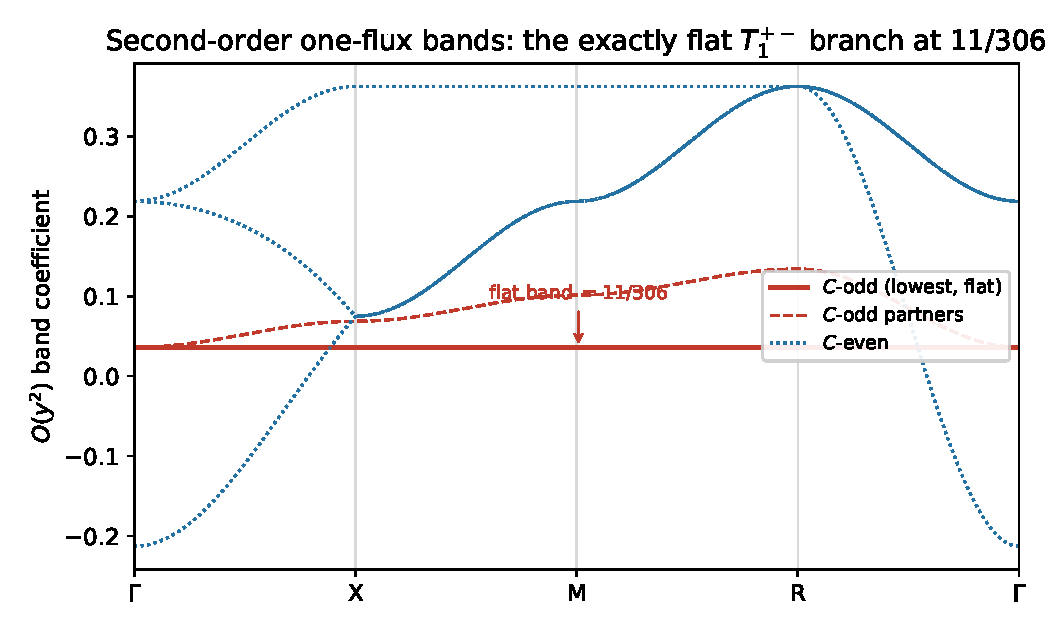
\includegraphics[width=0.86\textwidth]{PAPER_FLUX_fig_bands.pdf}
\caption{Second-order one-flux band coefficients (the $O(y^2)$ term) along
$\Gamma$--$X$--$M$--$R$--$\Gamma$. The lowest $C$-odd branch (solid) is exactly flat
at $11/306$ for every momentum---the Gauss-law $T_1^{+-}$ state of
Theorem~\ref{thm:flatband}; its dispersive $C$-odd partners (dashed) touch it
quadratically only at $\Gamma$. The $C$-even bands (dotted) disperse normally with
width $88/153$. Computed from the exact incidence symbols $\widetilde N(k)$ and
$A(k)$ of Theorem~\ref{thm:gausslaw}.}
\label{fig:bands}
\end{figure}

\begin{theorem}[Incidence factorization; Gauss law]\label{thm:gausslaw}
Let $N(k)$ and $B(k)$ be the unsigned and signed $3\times3$ Bloch incidence
symbols of the oriented plaquette-boundary map (each plaquette feeds its four
boundary links with incidence signs). With $u_j=1-e^{ik_j}$,
$v_j=1+e^{ik_j}$,
\begin{equation}
A(k)+4I=N(k)N(k)^\dagger,\quad \det N(k)=-2v_1v_2v_3;
\qquad
\Nt(k)+4I=B(k)B(k)^\dagger,\quad \det B(k)\equiv0 .
\end{equation}
Hence $\lambda(k)\in[-4,12]$ and $\mu(k)\in[-4,8]$ for the spectra of $A$
and $\Nt$, and the $C$-odd spectrum contains $\mu=-4$ \emph{at every} $k$:
the lowest $C$-odd band is the kernel of $B(k)^\dagger$, the states with zero
net signed amplitude into every link --- a lattice Gauss law.
\end{theorem}

\begin{proof}
$B$ is the boundary symbol: row $(\mu\nu)$ has entries
$e^{-ik_\nu/2}-e^{ik_\nu/2}$ and $e^{ik_\mu/2}-e^{-ik_\mu/2}$ in the link
channels $\mu,\nu$ (plaquette-center gauge) and $0$ in the transverse
channel; $BB^\dagger$ reproduces, entry by entry, the signed adjacency plus
$4I$ (each plaquette has four boundary links), which is verified symbolically.
Each row of $B$ is a linear combination of two link channels, and the three
rows involve the three channels cyclically with proportional weights; the
$3\times3$ determinant cancels identically (a two-term cancellation
$\propto \sin\tfrac{k_0}{2}\sin\tfrac{k_1}{2}\sin\tfrac{k_2}{2}$). The unsigned statement is the
same computation without signs.
\end{proof}

\begin{theorem}[$SU(N)$ shared-link universality]\label{thm:suniversal}
For every integer $N\geq3$, let $F$ denote the fundamental representation,
$C_F=(N^2-1)/(2N)$, and use the reduced shared-link normalization in which
the $SU(3)$ signed hop is $5/612$. The mixed-orientation fusion
$F\otimes\bar F=1\oplus\mathrm{Adj}$ and the like-orientation fusion
$F\otimes F=A_2\oplus S_2$ give
\begin{align}
w_1&=-\frac{2}{N(N-1)(N+1)},&
w_{\mathrm{Adj}}&=-\frac{2(N-1)(N+1)}{N(2N^2-1)},\notag\\
w_{A_2}&=-\frac{N-1}{(N+1)(2N-3)},&
w_{S_2}&=-\frac{N+1}{(N-1)(2N+3)}.
\label{eq:sunweights}
\end{align}
Consequently
\begin{align}
W_{\mathrm{mixed}}&=-\frac{2N^3}{(N^2-1)(2N^2-1)},\notag\\
W_{\mathrm{like}}&=-\frac{4N(N^2-2)}{(N^2-1)(4N^2-9)},\notag\\
\Sigma_N:=W_{\mathrm{like}}+W_{\mathrm{mixed}}
&=-\frac{2N(8N^4-19N^2+4)}{(N^2-1)(4N^2-9)(2N^2-1)},\notag\\
t_N:=W_{\mathrm{like}}-W_{\mathrm{mixed}}
&=\frac{2N(N^2-4)}{(N^2-1)(4N^2-9)(2N^2-1)}>0.
\label{eq:suntn}
\end{align}
The second-order $C$-odd operator therefore has the form
$H_{2,N}(k)=d_NI+t_N\Nt(k)$ for a scalar $d_N$. Since
$\Nt(k)$ has the exact eigenvalue $-4$ at every momentum, every $SU(N)$,
$N\geq3$, has a momentum-independent closed-surface eigenvalue
$d_N-4t_N$ at second order. Moreover,
\[
\Sigma_3=-\frac{481}{612},\qquad t_3=\frac5{612},\qquad
t_N=\frac{1}{4N^3}-\frac{1}{16N^5}+O(N^{-7}).
\]
\end{theorem}

\begin{proof}
After the six free-link integrations, the normalized shared-link tensor is
isotropic on the $N^2$-dimensional product space. If $P_R$ is the orthogonal
projector onto an irreducible channel $R$, its squared channel norm is
$\Tr P_R/N^2=d_R/N^2$. The six nonshared fundamental links contribute
$3C_F$ to the intermediate electric energy, while the fused shared link
contributes $C_R/2$; hence
\[
E_0=2C_F,\qquad E_R=3C_F+\frac{C_R}{2},\qquad
w_R=-\frac{d_R/N^2}{C_F+C_R/2}.
\]
Using
\[
d_1=1,\ C_1=0;\quad d_{\mathrm{Adj}}=N^2-1,\ C_{\mathrm{Adj}}=N;
\]
\[
d_{A_2}=\frac{N(N-1)}2,\ C_{A_2}=\frac{(N+1)(N-2)}N;\quad
 d_{S_2}=\frac{N(N+1)}2,\ C_{S_2}=\frac{(N-1)(N+2)}N
\]
gives \eqref{eq:sunweights}. Summing the two orientation families and
subtracting them gives \eqref{eq:suntn}. Every displayed factor in its
numerator and denominator is positive for $N\geq3$. The flat eigenvalue then
follows from Theorem~\ref{thm:gausslaw}; the asymptotic expansion is direct.
\end{proof}

\begin{theorem}[Exactly flat $T_1^{+-}$ band; compact localized states]
\label{thm:flatband}
The lowest $C$-odd band is exactly flat:
\begin{equation}
m_-(k,y)=\frac83+y+\frac{11}{306}\,y^2+O(y^3)
\qquad\text{for every }k\in\mathrm{BZ},
\end{equation}
since $\tfrac{7}{102}+\tfrac{5}{612}\,(-4)=\tfrac{11}{306}$. The dispersive
$C$-odd partners span coefficients $[\tfrac{11}{306},\tfrac{41}{306}]$,
touching the flat band quadratically at $k=0$. At rest the $C$-odd triplet
transforms as $T_1^{+-}$ of the cubic group with $C=-$ (axial-vector-like):
\emph{the $C$-odd one-plaquette sector contains no scalar at rest}.
\end{theorem}

\begin{theorem}[CLS, completeness, and $\partial\partial=0$]\label{thm:cls}
The consistently (Levi--Civita) oriented boundary of a single elementary
cube --- six faces with amplitudes $\pm1$ --- is an exact real-space
eigenvector of the signed adjacency at $\mu=-4$ with zero leakage onto any
plaquette off the cube. Its Bloch symbol $u(k)$ has
$|u(k)|^2=\sum_a\sin^2(k_a/2)$ and spans $\ker B(k)^\dagger$ for all
$k\neq0$. Flatness is the chain-complex identity
$\partial_2\partial_3=0$: every edge of the cube is shared by exactly two
faces with opposite induced orientation, so the signed face amplitudes cancel
on all twelve edges. Exactly, on an $L^3$ torus,
\begin{equation}
\dim\ker(\Nt+4I)\;=\;L^3+2\;=\;
\underbrace{\bigl(L^3\ \text{cube states},\ \text{rank }L^3-1\bigr)}_{
\text{one global relation }\sum_{\mathrm{cubes}}\psi=0}
\;\oplus\;
\underbrace{\bigl(3\ \text{rest states}\bigr)}_{\Nt(0)=-4I}.
\end{equation}
\end{theorem}

\begin{theorem}[The $C$-even band]\label{thm:ceven}
With the corrected hop \eqref{eq:tplus},
\begin{equation}
E_+(k,y)=\frac83-y+y^2\Bigl[\frac{223}{1020}-\frac{11}{306}\,\lambda(k)\Bigr],
\qquad \lambda(k)\in[-4,12],
\end{equation}
with band bottom $-\tfrac{217}{1020}$ at $k=0$ (the $A_1^{++}$, $0^{++}$
state), where $\lambda(k)=12-\tfrac43|k|^2+O(k^4)$ isotropically, hence
curvature $+\tfrac{22}{459}|k|^2y^2$ and effective mass $m^*=459/(44\,y^2)$;
band top $\tfrac{1109}{3060}$ at the zone faces; bandwidth
$16|t_+|=\tfrac{88}{153}$. At rest the triplet decomposes as
$A_1^{++}\oplus E^{++}$, with the $E^{++}$ doublet at the exact,
hop-independent coefficient $\tfrac{223}{1020}$ (it sits at $\lambda=0$).
\end{theorem}

\begin{remark}[An exactly immobile excitation]\label{rem:immobile}
The per-bond ratio is
\[
\frac{|t_-|}{|t_+|}=\frac{5/612}{11/306}=\frac5{22},
\]
and carries no immobility claim (this corrects Remark~6.4 of \cite{companion}, whose ratio
$5/481$ used the uncorrected hop). The immobility statement holds in exact
form: the lowest $C$-odd branch has bandwidth zero, while the full $C$-odd
manifold has width $\tfrac{5}{51}$ against the $C$-even bandwidth
$\tfrac{88}{153}$ (manifold-width ratio $15/88$). Both sectors factorize
through the link channel; the qualitative asymmetry is that
$\det N=-2v_1v_2v_3$ vanishes only on the zone faces $k_j=\pi$, while
$\det B\equiv0$ everywhere --- the $C$-even kernel is measure-zero, the
$C$-odd kernel is a whole band.
\end{remark}

\section{Third order: tromino vanishing and a rigid flat band}
\label{sec:thirdorder}

At $O(y^3)$ the new lattice geometry is the tromino: three plaquettes
pairwise sharing links.

\begin{lemma}[Bare-link lemma]\label{lem:barelink}
Every $O(y^3)$ tromino amplitude vanishes: each candidate three-plaquette
process leaves at least one boundary link in a nontrivial representation
unmatched (``bare''), and the corresponding Haar integral over that link is
zero. Trominoes first activate at $O(y^4)$.
\end{lemma}

Consequently the third-order effective Hamiltonian retains the second-order
(signed-adjacency, link-mediated) structure. The $C$-odd hopping is odd in the
shared-link orientation,
\[
T_3(s)=-T_3(-s),
\]
and the per-neighbor constants are computable on the abstract domino.

\begin{theorem}[Rigid flat band at third order]\label{thm:thirdorder}
The flat band of Theorem~\ref{thm:flatband} is rigid at $O(y^3)$:
\begin{equation}
m_-(k,y)=\frac83+y+\frac{11}{306}\,y^2-\frac{109151}{249696}\,y^3+O(y^4)
\qquad\text{for every }k,
\end{equation}
with
\begin{equation}
d_3=\frac{7}{32}+12\,\mathrm{leak}_3-4\,b_3=-\frac{109151}{249696},
\qquad
b_3=\frac{1975}{124848},\quad
\mathrm{leak}_3=-\frac{12331}{249696},
\end{equation}
where $\tfrac{7}{32}$ is the within-plaquette tower term \eqref{eq:towers},
$b_3$ the third-order $C$-odd hop and $\mathrm{leak}_3$ the per-neighbor
diagonal leakage; the dispersive $C$-odd top has cubic coefficient
$-\tfrac{61751}{249696}$. In the $C$-even sector,
\begin{equation}
m_+(0,y)=\frac83-y-\frac{217}{1020}\,y^2-\frac{54049}{520200}\,y^3+O(y^4),
\end{equation}
the band-top cubic coefficient is $\tfrac{471353}{1560600}$, and the diagonal
and hopping corrections obey the exact identity
$\mathrm{leak}^{\mathrm e}_n=T^{\mathrm e}_n$ at $n=2,3$ (two distinct
``$+3/4$'' mechanisms of equal value), so the $A_1^{++}$ correction at $k=0$
is (tower) $+\,24\,T^{\mathrm e}_n$ per order. From the certified band form,
the $E^{++}$ level acquires the cubic coefficient
$\tfrac{101}{200}+12\,T_3^{\mathrm e}=\tfrac{52163}{260100}$ and the
$C$-even curvature the correction
$+\tfrac43|T_3^{\mathrm e}|\,y^3=\tfrac{6335}{187272}\,y^3$.
\end{theorem}

\section{Robustness and exact fourth-order lifting}
\label{sec:robust}

\begin{theorem}[Link-mediated robustness]\label{thm:robust}
Let $H_{\mathrm{corr}}(k)=B(k)M(k)B(k)^\dagger$ be any correction whose
symbol factors through the link channel, with $M(k)$ an arbitrary Hermitian
symbol. Then $H_{\mathrm{corr}}$ annihilates the flat subspace:
\[
H_{\mathrm{corr}}(k)u(k)
=B(k)M(k)\bigl(B(k)^\dagger u(k)\bigr)=0.
\]
Consequently every link-mediated correction preserves the flat branch. A
separate $k$-independent scalar multiple of the identity may shift its energy
without producing dispersion. This explains the exact
second- and third-order rigidity.
\end{theorem}

\begin{theorem}[Sharpness]\label{thm:sharp}
The minimal corner-sharing, site-mediated symbol
\[
H_{\mathrm{corner}}(k)=\operatorname{diag}
\bigl(2\cos(k_0{+}k_1),2\cos(k_1{+}k_2),2\cos(k_0{+}k_2)\bigr)
\]
does not preserve the lower-order flat subspace:
$P_{\mathrm{flat}}H_{\mathrm{corner}}P_\perp\neq0$. Geometry alone does
not protect the band after site-mediated processes activate.
\end{theorem}

\subsection{The complete fourth-order kernel}

Let the exact translation-invariant fourth-order kernel be
$K_4(r)_{ba}$, where $a,b\in\{01,02,12\}$ label plaquette orientations and
$r\in\mathbb Z^3$ is the relative cell displacement. The recovered kernel
contains 189 nonzero rational records and obeys exact real-space
Hermiticity,
\[
K_4(r)_{ba}=K_4(-r)_{ab}.
\]
Its Bloch matrix is
\[
H_4(k)=\sum_rK_4(r)e^{ik\cdot r}.
\]
At zero momentum the full matrix is scalar,
\begin{equation}
H_4(0)=qI_3,
\qquad
q=-\frac{20721577909065127111}{7250590288602460800}.
\label{eq:qexact}
\end{equation}
This is both an exact kernel sum and the cubic-symmetry requirement on the
rest-frame $T_1^{+-}$ triplet.

For $k\neq0$ modulo reciprocal-lattice periodicity, use the cell/origin-gauge
flat vector
\begin{equation}
\psi(k)=
\begin{pmatrix}
e^{ik_2}-1\\
-(e^{ik_1}-1)\\
e^{ik_0}-1
\end{pmatrix},
\qquad
\|\psi(k)\|^2=2\sum_{i=0}^2X_i,
\qquad X_i=1-\cos k_i.
\label{eq:psicell}
\end{equation}
It spans the one-dimensional lower-order flat eigenspace away from the
threefold band touching at $\Gamma$.

\begin{theorem}[Exact fourth-order factorization]\label{thm:y4factor}
Define
\[
D(k)=\psi(k)^\dagger[H_4(k)-qI]\psi(k).
\]
The complete 189-record kernel gives the identity
\begin{equation}
D(k)=A\sum_iX_i^2+B\sum_{i<j}X_iX_j,
\qquad
A=\frac5{12},
\qquad
B=\frac{17607806155349}{275331901291200}.
\label{eq:Dfactor}
\end{equation}
Therefore the fourth-order coefficient of the branch that is flat through
third order is
\begin{equation}
c_4(k)=q+
\frac{A\sum_iX_i^2+B\sum_{i<j}X_iX_j}
{2\sum_iX_i},
\qquad k\neq\Gamma,
\label{eq:c4closed}
\end{equation}
with continuous value $c_4(\Gamma)=q$.
\end{theorem}

\begin{proof}
Contracting the exact Laurent-polynomial kernel with \eqref{eq:psicell}
leaves 25 nonzero frequencies. Hermiticity and cubic symmetry reduce them to
three cosine orbits: unit-axis frequencies, double-axis frequencies, and the
six pair frequencies. Thus
\[
D=C+a\sum_i\cos k_i+d\sum_i\cos2k_i
+b\sum_{i<j}\{\cos(k_i+k_j)+\cos(k_i-k_j)\}.
\]
The exact kernel coefficients satisfy
\[
C+3a+3d+6b=0,
\qquad 2d=\frac5{12},
\qquad 2b=B,
\qquad -a-4d-4b=0.
\]
The first identity is $D(0)=0$; the last is the cancellation of the term
linear in $X_i=1-\cos k_i$, equivalently the continuity of
$D(k)/(2\sum_iX_i)$ with value zero at $\Gamma$. Substitution of
$\cos2k_i=1-4X_i+2X_i^2$ and
$\cos(k_i+k_j)+\cos(k_i-k_j)=2(1-X_i)(1-X_j)$ gives
\eqref{eq:Dfactor}. Equation~\eqref{eq:c4closed} follows from
$\|\psi\|^2=2\sum_iX_i$. At $\Gamma$, \eqref{eq:qexact} gives the
continuous value directly.
\end{proof}

The complete strong-coupling branch through fourth order is consequently
\begin{equation}
m_-(k,y)=\frac83+y+\frac{11}{306}y^2
-\frac{109151}{249696}y^3+c_4(k)y^4+O(y^5).
\label{eq:branch4}
\end{equation}

\begin{theorem}[Exact real-space sum of squares]\label{thm:y4sos}
Let $C=\partial_3$ map scalar cube amplitudes to their consistently oriented
plaquette boundaries in the cell/origin gauge, so its Fourier symbol is
$\psi(k)$ in \eqref{eq:psicell}. Let $T_i$ translate cube amplitudes by one
cell and define
\[
\nabla_i=T_i-I,
\qquad
L_i=\nabla_i^\dagger\nabla_i=2I-T_i-T_i^{-1}.
\]
Then the complete fourth-order kernel obeys the exact local operator identity
\begin{equation}
\boxed{
C^\dagger(H_4-qI)C
=\frac{A}{4}\sum_iL_i^2
+\frac{B}{4}\sum_{i<j}L_iL_j
}
\label{eq:sosoperator}
\end{equation}
with $A,B$ from \eqref{eq:Dfactor}. Equivalently,
\begin{equation}
C^\dagger(H_4-qI)C
=\frac5{48}\sum_iL_i^2
+\frac{17607806155349}{1101327605164800}
\sum_{i<j}(\nabla_i\nabla_j)^\dagger
               (\nabla_i\nabla_j).
\label{eq:sosexplicit}
\end{equation}
The scalar numerator operator $Q=C^\dagger(H_4-qI)C$ is the 25-point stencil
\begin{align}
(Q\phi)_x={}&w_0\phi_x
+w_1\sum_i(\phi_{x+e_i}+\phi_{x-e_i})
+w_2\sum_i(\phi_{x+2e_i}+\phi_{x-2e_i})\notag\\
&+w_d\sum_{i<j}\sum_{\sigma,\tau=\pm1}
\phi_{x+\sigma e_i+\tau e_j},
\label{eq:sosstencil}
\end{align}
where
\begin{equation}
\begin{split}
w_0&=\frac{189690244462349}{91777300430400},\\
w_1&=-\frac{132329431693349}{275331901291200},\\
w_2&=\frac5{48},\qquad
w_d=\frac{17607806155349}{1101327605164800},
\end{split}
\label{eq:sosweights}
\end{equation}
and $w_0+6w_1+6w_2+12w_d=0$.

The cube-boundary states have Gram operator
\begin{equation}
G=C^\dagger C=\sum_iL_i.
\label{eq:cubegram}
\end{equation}
Consequently the physical lift is the generalized eigenproblem
\begin{equation}
Q\phi=\lambda G\phi,
\qquad
\lambda(k)=c_4(k)-q
=\frac{A\sum_iX_i^2+B\sum_{i<j}X_iX_j}
       {2\sum_iX_i}.
\label{eq:sosgeneralized}
\end{equation}
\end{theorem}

\begin{proof}
The symbol of $L_i$ is
$|e^{ik_i}-1|^2=2X_i$. Hence the Fourier symbol of the right side of
\eqref{eq:sosoperator} is
\[
\frac A4\sum_i(2X_i)^2
+\frac B4\sum_{i<j}(2X_i)(2X_j)
=A\sum_iX_i^2+B\sum_{i<j}X_iX_j,
\]
which equals the exact contracted symbol $D(k)$ by
Theorem~\ref{thm:y4factor}. Since both sides are finite-range
translation-invariant operators, equality of their Laurent symbols proves the
real-space identity. Expanding $L_i^2$ and $L_iL_j$ gives
\eqref{eq:sosstencil}--\eqref{eq:sosweights}. Equation~\eqref{eq:cubegram}
follows from the definition of $C$, and division by its symbol
$2\sum_iX_i$ gives \eqref{eq:sosgeneralized}. The exact certificate also
contracts the 189-record kernel directly and obtains the same 25 rational
coefficients with zero residual.
\end{proof}

\begin{remark}[Geometric carriers of fourth-order mobility]
For a localized cube amplitude, $L_i$ creates the axial three-cube pattern
$(-1,2,-1)$, while $\nabla_i\nabla_j$ creates a planar four-cube
checkerboard $(+1,-1,-1,+1)$. Equation~\eqref{eq:sosexplicit} states that the
first mobility of the closed-surface excitation is exactly the positive
weighted norm of these two local deformations.
\end{remark}

\begin{theorem}[Exact global band edges]\label{thm:y4edges}
Modulo reciprocal-lattice periodicity, $\Gamma=(0,0,0)$ is the unique global
minimum of $c_4(k)$ and $R=(\pi,\pi,\pi)$ is the unique global maximum.
The exact fourth-order bandwidth is
\begin{equation}
\Delta W_4=c_4(R)-c_4(\Gamma)
=A+B
=\frac{132329431693349}{275331901291200}.
\label{eq:bandwidth4}
\end{equation}
\end{theorem}



\begin{proof}
For $k\neq\Gamma$, the variables satisfy $X_i\in[0,2]$ and
$S=\sum_iX_i>0$. Since $A>0$, $B>0$, and
$\sum_iX_i^2>0$, equation~\eqref{eq:Dfactor} gives $D(k)>0$. Hence
$c_4(k)>q=c_4(\Gamma)$.

For the upper edge, write
$Q=\sum_iX_i^2$ and $R_2=\sum_{i<j}X_iX_j$. On the cube
$0\leq X_i\leq2$,
\[
Q\leq2S,
\qquad R_2\leq2S.
\]
For the second inequality set $x_i=X_i/2$; then
\[
(x_0+x_1+x_2)-(x_0x_1+x_0x_2+x_1x_2)
=x_0(1-x_1)+x_1(1-x_2)+x_2(1-x_0)\geq0.
\]
Therefore $c_4(k)-q\leq A+B$. Equality away from $\Gamma$ requires
$x_0=x_1=x_2=1$, hence $X_0=X_1=X_2=2$, which is precisely
$R=(\pi,\pi,\pi)$ modulo $2\pi$.
\end{proof}

\begin{proposition}[Kinematic generic-$N$ factorization]
\label{prop:sunh4conditional}
Fix an integer $N\geq3$ and define
\[
D_N(k)=\psi(k)^\dagger[H_{4,N}(k)-q_NI]\psi(k).
\]
Suppose the exact rank-$N$ kernel passes the group-independent gates of
Hermiticity, cubic covariance, independent-reflection symmetry, the same final
displacement support as the $SU(3)$ kernel, and
$H_{4,N}(0)=q_NI$. Then
\[
D_N(k)=A_N\sum_iX_i^2+B_N\sum_{i<j}X_iX_j.
\]
Writing $q_N,c_X,c_M,c_R$ for the exact fourth-order branch coefficients at
$\Gamma,X,M,R$, respectively,
\[
A_N=c_X-q_N,
\qquad
B_N=2(c_M-c_X)=c_R-c_X,
\qquad
c_R=2c_M-c_X.
\]
The last equality is a hard consistency gate on any generic-$N$ computation.
The proposition is purely kinematic. Theorem~\ref{thm:sunfull} verifies its hypotheses and the signs of
$A_N,B_N$ throughout the stable range $N\geq7$, while
Theorem~\ref{thm:sunallband} closes the band shape at $N=3,4,5,6$.
\end{proposition}

\begin{proof}
The final displacement support and cubic/reflection symmetries restrict $D_N$
to a constant, a term proportional to $S=\sum_iX_i$, and the two quadratic
cubic invariants $Q=\sum_iX_i^2$ and
$R_2=\sum_{i<j}X_iX_j$. Since $\psi(k)=O(k)$ and
$H_{4,N}(k)-q_NI=O(k)$, analyticity gives $D_N(k)=O(|k|^3)$.
Independent reflections make $D_N$ even, hence in fact
$D_N(k)=O(|k|^4)$. The constant and quadratic Taylor terms therefore vanish,
leaving $A_NQ+B_NR_2$. Evaluating $(A_NQ+B_NR_2)/(2S)$ at $X$, $M$, and $R$
gives $A_N$, $A_N+B_N/2$, and $A_N+B_N$, respectively, yielding the stated
reconstruction identities.
\end{proof}

The high-symmetry values are
\begin{align}
c_4(\Gamma)&=-\frac{20721577909065127111}{7250590288602460800},\notag\\
c_4(X)&=-\frac{17700498622147435111}{7250590288602460800},\notag\\
c_4(M)&=-\frac{4367164159624988707}{1812647572150615200},\notag\\
c_4(R)&=-\frac{3447362930970494909}{1450118057720492160}.
\label{eq:bandpoints4}
\end{align}

\begin{figure}[t]
\centering
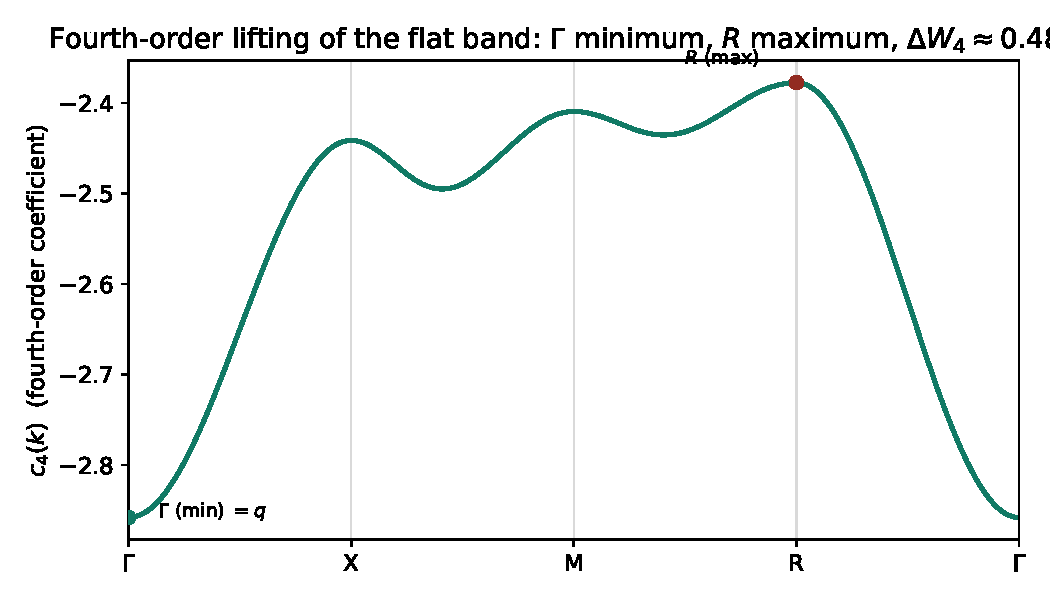
\includegraphics[width=0.86\textwidth]{PAPER_FLUX_fig_c4.pdf}
\caption{The fourth-order coefficient $c_4(k)$ of equation~\eqref{eq:c4closed}
along $\Gamma$--$X$--$M$--$R$--$\Gamma$, exhibiting the exact global structure of
Theorem~\ref{thm:y4edges}: a unique minimum at $\Gamma$ (value $q$), a unique maximum
at $R$, and the parameter-free bandwidth $\Delta W_4=A+B\approx0.4806$. This is the
first nonzero dispersion of the closed-surface branch, exactly immobile through
$O(y^3)$.}
\label{fig:c4}
\end{figure}

\begin{proposition}[Band-edge regularity and curvature]\label{prop:y4curvature}
For $k=tn$ with $|n|=1$,
\begin{equation}
c_4(tn)-q
=\frac{t^2}{4}
\left[A\sum_i n_i^4+B\sum_{i<j}n_i^2n_j^2\right]+O(t^4).
\label{eq:gammacurv}
\end{equation}
The directional coefficient ranges from
\[
\kappa_{\mathrm{diag}}=\frac{A+B}{12}
=\frac{132329431693349}{3303982815494400}
\]
on a body diagonal to
\[
\kappa_{\mathrm{axis}}=\frac{A}{4}=\frac5{48}
\]
on a coordinate axis. Thus the $\Gamma$ lift is quadratic but not the
restriction of a single Hessian. At the upper edge,
\begin{equation}
c_4(R+\delta)=c_4(R)
-\frac{132329431693349}{3303982815494400}|\delta|^2
+O(|\delta|^4),
\label{eq:Rcurv}
\end{equation}
so the $R$ curvature is isotropic and negative.
\end{proposition}

\begin{proof}
Near $\Gamma$, $X_i=t^2n_i^2/2+O(t^4)$; insertion into
\eqref{eq:c4closed} gives \eqref{eq:gammacurv}. Since
$\sum_i n_i^4\in[1/3,1]$,
$\sum_{i<j}n_i^2n_j^2=(1-\sum_i n_i^4)/2$, and $A-B/2>0$, the stated
extrema follow.
If a Hessian existed at $\Gamma$, cubic symmetry would force it to be a
scalar multiple of the identity, contradicting the two distinct directional
coefficients. Near $R$, $X_i=2-\delta_i^2/2+O(\delta_i^4)$; expanding the
ratio in \eqref{eq:c4closed} gives \eqref{eq:Rcurv}.
\end{proof}


\subsection{Stable-rank $SU(N\geq7)$ fourth-order reduction}
\label{subsec:sunstable}

\begin{theorem}[Stable-rank local-invariant and denominator theorem]
\label{thm:sunstable}
For the complete connected fourth-order geometry, the maximum local tensor
degree is six. For every integer $N\geq7$, all local $SU(N)$ singlets are
therefore exactly balanced in fundamental and antifundamental degree; no
independent determinant/epsilon sectors occur. The local Haar integrations
reduce to the three balanced families $(1,1)$, $(2,2)$, and $(3,3)$, with
\[
\operatorname{Wg}_1(e)=\frac1N,
\]
\[
\operatorname{Wg}_2(e)=\frac1{N^2-1},\qquad
\operatorname{Wg}_2((12))=-\frac1{N(N^2-1)},
\]
and
\[
\operatorname{Wg}_3(e)=\frac{N^2-2}{N(N^2-1)(N^2-4)},
\]
\[
\operatorname{Wg}_3((12))=-\frac1{(N^2-1)(N^2-4)},\qquad
\operatorname{Wg}_3((123))=\frac2{N(N^2-1)(N^2-4)}.
\]
The stable mixed-tensor irreducible channels are indexed by bipartitions
$(\lambda,\mu)$, with
\[
C_2(\lambda,\mu)=
\frac{N^2(|\lambda|+|\mu|)
+N[\kappa(\lambda)+\kappa(\mu)]
-(|\lambda|-|\mu|)^2}{2N},
\qquad
\kappa(\lambda)=\sum_i\lambda_i(\lambda_i+1-2i).
\]
Consequently every electric denominator is an explicit rational function of
$N$. Exact enumeration yields the counts in Table~\ref{tab:sunstable}; there
are 94 distinct denominator polynomials and none has an accidental integer
root for $N\geq7$. Evaluating the stable bipartition engine at $N=3$ agrees
with the existing $SU(3)$ Dynkin-label engine on all 140 balanced token
signatures.
\end{theorem}

\begin{proof}
A local invariant with $n_f$ fundamental and $n_{\bar f}$ antifundamental
indices requires
$n_f-n_{\bar f}\equiv0\pmod N$. The verified local degree bound gives
$|n_f-n_{\bar f}|\leq6$; for $N\geq7$ this congruence is equivalent to
$n_f=n_{\bar f}$. The Weingarten coefficients are the exact inverses of the
permutation Gram matrices through degree three. Stable mixed-tensor branching
then gives the displayed bipartition Casimir. The geometry counts,
denominator classification, absence of integer roots, and 140-signature
regression are exact integer and symbolic gates in the certificate described
in Appendix~\ref{app:verification}.
\end{proof}


\begin{theorem}[Exact stable-rank local walled-Brauer projectors]
\label{thm:wbprojectors}
For every compact balanced token family of local degree
$r\in\{1,2,3\}$, let the invariant pairing basis be indexed by
$\sigma\in S_r$ and let
\[
G_{\sigma\tau}=N^{\#\operatorname{cycles}(\sigma^{-1}\tau)}.
\]
For each mixed-tensor branching path $p$, there is an exact rank-one action
matrix $Q_p$ over $\mathbb Q(N)$. In the $r!$-dimensional pairing basis, its
channel-resolved Haar dyad is
\[
D_p=Q_pG^{-1}.
\]
The complete set satisfies
\[
Q_p^2=Q_p,\qquad \operatorname{tr}Q_p=1,\qquad
Q_p^TG=GQ_p,\qquad C_{\rm total}Q_p=0,
\]
\[
Q_pQ_{p'}=0\quad(p\ne p'),\qquad
\sum_pQ_p=I,\qquad \sum_pD_p=G^{-1},\qquad D_p^T=D_p.
\]
Exact enumeration gives 28 compact token families, 134 distinct path
projectors, 730 spectral factors, and 330 path instances across the 140
balanced six-event signatures. All 746 Weingarten-entry gates, 1,338
projector-matrix gates, and 140 Stage-1 channel-history regressions pass.
Consequently the local Stage-3C carrier/projector layer is closed over
$\mathbb Q(N)$ for every integer $N\geq7$.
\end{theorem}

\begin{proof}
Nested partial-Casimir spectral factors construct the path action matrices in
the pairing basis. Direct symbolic reduction over $\mathbb Q(N)$ verifies the
displayed projector, Gram-adjoint, orthogonality, completeness, and total-Casimir
identities. Multiplication by the exact Weingarten inverse gives $D_p$ and the
path sum $\sum_pD_p=G^{-1}$. The complete serialized matrices and the
independent gate re-evaluation are described in
Appendix~\ref{app:verification}.
\end{proof}

\begin{table}[t]
\centering
\small
\begin{tabular}{lr@{\qquad}lr}
\toprule
quantity & count & quantity & count \\
\midrule
connected supports & 182440 & candidate support/output pairs & 895524 \\
stable support/output classes & 439 & canonical ordered words & 4171 \\
exact-balance sign assignments & 33500 & charge-conjugation orbits & 16750 \\
unique balanced signatures & 140 & symbolic energy signatures & 37500 \\
resonant signatures & 17073 & nonresonant signatures & 20427 \\
distinct denominator polynomials & 94 & accidental roots, $N\geq7$ & 0 \\
compact token families & 28 & unique path projectors & 134 \\
six-event path instances & 330 & spectral factors & 730 \\
Weingarten-entry gates & 746 & projector-matrix gates & 1338 \\
trace topologies & 3850 & global fusion paths & 35130 \\
$q_N$ topologies / paths & 2290 / 27202 & $q_N$ denominator classes & 167 \\
$A_N$ topologies / paths & 406 / 950 & $A_N$ energy groups & 140 \\
$B_N$ topologies / paths & 2328 / 13096 & $B_N$ energy groups & 743 \\
\bottomrule
\end{tabular}
\caption{Exact stable-rank fourth-order geometry, local-projector, and global-contraction counts.}
\label{tab:sunstable}
\end{table}

\begin{theorem}[Stable-rank full fourth-order coefficient theorem]
\label{thm:sunfull}
For every integer $N\geq7$, the complete global Stage-3G trace-index
contraction passes the kernel hypotheses of
Proposition~\ref{prop:sunh4conditional}. With $X_i=1-\cos k_i$,
\[
D_N(k)=\psi(k)^\dagger[H_{4,N}(k)-q_NI]\psi(k)
=A_N\sum_iX_i^2+B_N\sum_{i<j}X_iX_j,
\]
and, for $k\ne\Gamma$,
\[
c_{4,N}(k)=q_N+
\frac{A_N\sum_iX_i^2+B_N\sum_{i<j}X_iX_j}
{2\sum_iX_i}.
\]
Set $z=N^2$. The exact coefficients are
\[
q_N=-\frac{2}{3N}\frac{Q_{32}(z)}{D_{34}(z)},
\qquad
A_N=\frac{640}{N(N^2-1)^3},
\qquad
B_N=\frac{P_{17}(z)}{N R_{20}(z)},
\]
where $Q_{32},D_{34}$ are the exact integer polynomials in the supplementary
$q_N$ ledger and $P_{17},R_{20}$ are displayed in
Appendix~\ref{app:compactpolys}. For every integer $N\geq7$,
\[
q_N<0,\qquad A_N>0,\qquad B_N>0.
\]
Modulo reciprocal-lattice periodicity, $\Gamma$ is therefore the unique
global minimum of $c_{4,N}$, $R=(\pi,\pi,\pi)$ is the unique global maximum,
and
\[
\boxed{\Delta c_{4,N}=c_{4,N}(R)-c_{4,N}(\Gamma)=A_N+B_N>0.}
\]
The exact contraction census is 3,850 trace topologies and 35,130 global
fusion paths. The $q_N$, $A_N$, and $B_N$ sectors receive respectively
27,202, 950, and 13,096 nonzero path contributions.
\end{theorem}

\begin{proof}
The local projectors of Theorem~\ref{thm:wbprojectors} are contracted through
the oriented trace boundaries of all 4,171 ordered words by exact
partition/loop elimination. The resulting fixed-rank kernels have 189
real-space entries, satisfy Hermiticity and cubic covariance, obey
$H_{4,N}(0)=q_NI$, and give identical values of
$2[c_{4,N}(M)-c_{4,N}(X)]$ and $c_{4,N}(R)-c_{4,N}(X)$. Thus
Proposition~\ref{prop:sunh4conditional} yields the displayed two-invariant
form.

For $q_N$, every factor of $D_{34}(z)$ is positive for $z=N^2\geq49$, while
\[
Q_{32}(z)=\sum_{j=0}^{32}b_j\binom{z-49}{j},\qquad b_j>0.
\]
Hence $q_N<0$. The sign of $A_N$ is immediate. The original 74-term
structured expression for $B_N$ reduces exactly to the displayed compact
form after cancellation of
$(4N-5)(4N+5)(4N^2-3)$. Every factor of $R_{20}(z)$ is positive for
$z\geq49$, and
\[
P_{17}(z)=\sum_{j=0}^{17}a_j\binom{z-49}{j},\qquad a_j>0,
\]
so $B_N>0$. Exact fixed-rank contractions for $N=7,\ldots,18$, including the
unused $N=18$ holdout, match the symbolic formulas. The global extrema and
bandwidth then follow from the cube inequalities used in
Theorem~\ref{thm:y4edges}.
\end{proof}

\begin{corollary}[Stable-rank large-$N$ collapse]
\label{cor:sunlargeN}
The exact compact forms give
\[
q_N=-\frac{227}{N^5}+O(N^{-7}),\qquad
A_N=\frac{640}{N^7}+O(N^{-9}),\qquad
B_N=\frac{6170}{9N^7}+O(N^{-9}).
\]
Consequently
\[
\frac{B_N}{A_N}\longrightarrow\frac{617}{576},\qquad
\Delta c_{4,N}=\frac{11930}{9N^7}+O(N^{-9}).
\]
\end{corollary}

\begin{theorem}[Fourth-order band shape for all non-pseudoreal ranks]
\label{thm:sunallband}
For $SU(3)$,
\[
A_3=\frac5{12},\qquad
B_3=\frac{17607806155349}{275331901291200}.
\]
For every integer $N\geq4$,
\[
A_N=\frac{640}{N(N^2-1)^3},\qquad
B_N=\frac{P_{17}(N^2)}{N R_{20}(N^2)}.
\]
For every integer $N\geq3$,
\[
A_N>0,\qquad B_N>0.
\]
Therefore $\Gamma$ is the unique global minimum, $R$ is the unique global
maximum, and
\[
\boxed{\Delta c_{4,N}=A_N+B_N>0}
\]
for every non-pseudoreal $SU(N)$.
\end{theorem}

\begin{proof}
The case $N=3$ is Theorem~\ref{thm:y4factor}. For $N\geq7$ the statement is
Theorem~\ref{thm:sunfull}. A fresh exact $N$-ality scan gives the following
finite exceptional-rank reductions. At $N=4$ there are 312 additional
determinant-sector assignments, or 156 charge-conjugation orbits. Only 40
exceptional ordered words enter the 64-key $A/B$ target. Their contraction
contains 48 active trace topologies in nine equal-amplitude classes: every
$A$-functional coefficient vanishes individually, while each $B$ class has
equal multiplicities of coefficients $+8$ and $-8$. Hence
$\Delta A_4=\Delta B_4=0$. At $N=5$ no determinant assignment occurs anywhere
in the complete fourth-order geometry. At $N=6$ one determinant
charge-conjugation orbit occurs, but it is absent from all 64 entries defining
$A_6$ and $B_6$. Thus the balanced compact formulas hold at $N=4,5,6$.
Their positivity is checked by exact substitution, completing the proof.
\end{proof}

\begin{theorem}[$SU(2)$ exclusion]\label{thm:su2excl}
In pure $SU(2)$ gauge theory there is no one-flux $T_1^{+-}$ branch. Every
fundamental matrix obeys $U^*=\varepsilon U\varepsilon^{-1}$ with
$\varepsilon=i\sigma_2$; the constant gauge transformation $g_x=\varepsilon$ at
every vertex sends $U_{xy}\mapsto U_{xy}^*$, so charge conjugation is a gauge
transformation and acts trivially on the physical Hilbert space. Hence $C=I$,
$P_{C=-}=0$, and $q_2,A_2,B_2$ are undefined. The band-shape theorem domain
$N\geq3$ is therefore maximal.
\end{theorem}

\begin{remark}[Determinant offsets at exceptional rank]
The common offset $q_3$ is known from the rank-specific $SU(3)$ kernel, and $q_5$
(fourth order, $SU(5)$) is given by the balanced formula in
Theorem~\ref{thm:sunfull}. The determinant-sector corrections to the remaining
exceptional offsets are $\Delta q_4=-304746539168/160249753125$ and
$\Delta q_6=6/343$, both scalar on the closed-surface branch with
$\Delta A=\Delta B=0$ ($SU(5)$ has no determinant sector). They shift only the
rest energy and do not enter the extrema or bandwidth theorem.
\end{remark}

\section{SU(3) fifth order and the scale-matched mass ratio}
\label{sec:fifth}

Everything above is fourth order and holds for all ranks $N\geq3$. The same
$SU(3)$ machinery extends to fifth order in $y$. The fifth-order kernel is again a
$189$-record real-space object, and the projected coefficient has the
\emph{identical} two-invariant form as fourth order.

\begin{theorem}[Fifth-order $SU(3)$ band]\label{thm:fifth}
For $X_i=1-\cos k_i$, $S=\sum_iX_i$, $Q=\sum_iX_i^2$, $R=\sum_{i<j}X_iX_j$,
\[
c_5(k)=q_5+\frac{A_5\,Q+B_5\,R}{2S},
\qquad
A_5=\frac{313}{240},\quad
B_5=\frac{1881863087742908605903793}{1652932248975967181040000},
\]
\[
q_5=-\frac{866236750503342026253096691057}{1169668083793811403447133488000}
\approx-0.740583386437.
\]
Both shape coefficients are positive ($A_5\approx1.3042$, $B_5\approx1.1385$), so
$\Gamma$ is the unique minimum and $R$ the unique maximum of $c_5$, with exact
bandwidth
\[
\Delta c_5=A_5+B_5=\frac{4037562229115732471176793}{1652932248975967181040000}
\approx2.442666.
\]
\end{theorem}

The parity anchors satisfy the same exact consistency gate $c_R=2c_M-c_X$ and the
extraction relations $A_5=c_X-q_5$, $B_5=2(c_M-c_X)=c_R-c_X$, both checked to agree.
The flat-band picture therefore persists through $O(y^5)$; what changes is only
magnitude---the fifth-order shape coefficients are $O(1)$, so the band is no longer
approximately flat at this order. The complete rest-mass series is
\begin{equation}
m_{1^{+-}}(y)=\frac83+y+\frac{11}{306}y^2-\frac{109151}{249696}y^3
-\frac{20721577909065127111}{7250590288602460800}y^4
-\frac{866236750503342026253096691057}{1169668083793811403447133488000}y^5
+O(y^6).
\label{eq:restseries5}
\end{equation}
The fifth-order contraction is substantially larger than fourth: $6{,}676{,}658$
connected five-insertion supports, $29{,}366$ canonical ordered words, $524{,}823$
global path contractions, and $189$ nonzero kernel records; the new local sectors
are $(4,1)$ and $(5,2)$.

\subsection{Project-native string tension and the scale-matched ratio}
\label{sec:ratio}

The static-flux (torelon) strong-coupling expansion gives the Hamiltonian string
tension in the same variable $y=\beta/6$. The connected-support engine reproduces,
$L$-independently and exact against the Kogut--Pearson--Shigemitsu (KPS) table
through fourth order,
\[
\sigma(y)=\frac23-\frac{22}{153}y^2-\frac{61}{408}y^3
-\frac{737327120374220449}{7250590288602460800}y^4+O(y^5).
\]
The conversion to the KPS variable $x=2y$ is the single bridge
$\sigma(y)=\tfrac12W(2y)$; this sign convention---in particular the \emph{negative}
odd coefficient $\sigma_3=-61/408$---is forced by the native engine (the alternative
$\tfrac12W(-2y)$ gives $+61/408$ and is excluded). The fifth-order tension $\sigma_5$
has since been reproduced by an independent \emph{native} first-principles computation
(Appendix~\ref{app:nativesigma}): an exact $SU(3)$ torelon strong-coupling engine that,
unlike the adjoint-sector contraction, resolves the determinant/$\varepsilon$ (triality)
sector that carries all odd orders. It reproduces $\sigma_2,\sigma_3$ in exact rational
arithmetic and now determines $\sigma_5$ in \emph{exact finite-field} arithmetic: computed
modulo seven independent primes, CRT-combined ($189$-bit modulus), and rational-reconstructed
with no literature input (Appendix~\ref{app:nativesigma}), coinciding with the historical KPS
value. Thus $\sigma_5$ is exact, not merely a KPS target. The sixth tension $\sigma_6$ remains an exact
KPS historical target (its native evaluation is of larger, external-memory scale). The scale-matched ratio is then
\begin{equation}
\frac{m_{1^{+-}}(y)}{\sqrt{\sigma(y)}}=\sqrt6\sum_{n=0}^{5}c_ny^n+O(y^6),
\qquad
\begin{aligned}
&c_0=\tfrac43,\quad c_1=\tfrac12,\quad c_2=\tfrac{11}{68},\quad
c_3=-\tfrac{7559}{499392},\\
&c_4=-\tfrac{15752822901180179}{12642703205932800},\quad
c_5=-\tfrac{10670728893034386567182468628311}{46786723351752456137885339520000},
\end{aligned}
\label{eq:ratio5}
\end{equation}
re-derived independently from the rest-mass and string-tension series. The
sixth-order ratio coefficient is fixed up to one unknown, $c_6=\tfrac12m_6+K$ with
$K$ exact, so only the sixth-order rest mass $m_6$ is missing to reach $O(y^6)$.

\begin{remark}[Sixth order: a provisional internal value]
The global $\Gamma$-contraction has since been carried out as an exact
external-memory computation over the full $247{,}326{,}161$-support census
($3{,}094{,}806$ canonical ordered words, $205{,}699$ nonzero $\Gamma$-point
topology blocks, $10{,}907{,}384$ global local-path choices), summed as $229$
exact rational shards. In the project convention it gives
\[
m_6=-\frac{156998370765216917515896262601525405897211506214753116643443873}
{4880681791275629050759264798095652027950878794719744000000}
\approx-32167.30,
\]
and correspondingly, for the ratio $m_{1^{+-}}/\sqrt\sigma=\sqrt6\sum_n c_nu^n$,
\[
c_6=-\frac{4270353824428899200786427191557487127249971701568661364147801}
{265509089445394220361304005016403470320527806432754073600}\approx-16083.64 .
\]
This is exact \emph{within the enumerated one-flux des-Cloizeaux construction}.
Three internal gates support it: the identical $\Gamma$-reduction reproduces
$q_5$ exactly; the $32$ resonance-pattern folded weights agree with an
independent Rayleigh--Schr\"odinger recurrence; and the dominant
high-multiplicity anchor (folded weight $-243/16384$, $\Gamma$-multiplicity
$65208$, eight blocks summing to $-1980693/256$) is reproduced here independently
by the folded-weight module used for the $\sigma_5$ certificate, which matches the
contraction's fold formula on every test vector. An independent reimplementation now confirms the computational primitives:
a weight-blocked Casimir-nullspace Haar engine reproduces the local singlet
projectors \emph{matrix-exactly} for all order-four signatures and matches the
singlet dimension and cumulative-Casimir histories for every triality family
through degree eight (the order-six carriers, including the determinant sectors);
the $\sigma_5$-certified des-Cloizeaux module reproduces the contraction's folded
weights exactly; and the full order-four pipeline was rerun from scratch,
regenerating $q_4$. The result is nonetheless retained as \textbf{provisional}:
what remains for theorem-level promotion is an independent re-derivation of the
order-six \emph{geometry census} (the $247{,}326{,}161$-support enumeration and its
$\Gamma$ multiplicities), which is external-memory scale. The coefficient is
anomalously large relative to $q_2,\dots,q_5$; the audit traces this to a small
family of high-multiplicity, low-path-dimension $\Gamma$ blocks rather than to
numerical instability, and the magnitude lives in those order-six multiplicities,
not in the (now independently verified) color or fold layers.
\end{remark}

\section{Numerical summary and discussion}
\label{sec:numbers}

Table~\ref{tab:lowerbands} collects the exact lower-order data. These entries
are unchanged from the third-order certificate chain.

\begin{table}[ht]
\centering
\scriptsize
\begin{tabular}{lll}
\toprule
quantity & exact & decimal \\
\midrule
$C$-odd flat branch, $O(y)$ / $O(y^2)$ / $O(y^3)$ &
$+1$; $+11/306$; $-109151/249696$ &
$1$; $0.0359477$; $-0.4371356$ \\
$C$-odd dispersive top, $O(y^2)$ / $O(y^3)$ &
$41/306$; $-61751/249696$ & $0.1339869$; $-0.2473048$ \\
$C$-odd manifold width ($y^2$) & $5/51$ & $0.0980392$ \\
$A_1^{++}$ bottom, $O(y)$ / $O(y^2)$ / $O(y^3)$ &
$-1$; $-217/1020$; $-54049/520200$ &
$-1$; $-0.2127451$; $-0.1039004$ \\
$E^{++}$ level, $O(y^2)$ / $O(y^3)$ &
$223/1020$; $52163/260100$ & $0.2186275$; $0.2005498$ \\
$C$-even bandwidth ($y^2$) & $88/153$ & $0.5751634$ \\
$C$-even effective mass & $459/(44y^2)$ & $10.43182/y^2$ \\
per-bond ratio $|t_-|/|t_+|$ & $5/22$ & $0.2272727$ \\
\bottomrule
\end{tabular}
\caption{Exact one-flux data through third order. The lowest $C$-odd branch
is flat at every momentum through the displayed orders.}
\label{tab:lowerbands}
\end{table}

The new fourth-order data are summarized in Table~\ref{tab:y4band}.

\begin{table}[ht]
\centering
\scriptsize
\begin{tabular}{lll}
\toprule
quantity & exact & decimal \\
\midrule
$c_4(\Gamma)$ &
$-20721577909065127111/7250590288602460800$ & $-2.857915988115$ \\
$c_4(X)$ &
$-17700498622147435111/7250590288602460800$ & $-2.441249321448$ \\
$c_4(M)$ &
$-4367164159624988707/1812647572150615200$ & $-2.409273720232$ \\
$c_4(R)$ &
$-3447362930970494909/1450118057720492160$ & $-2.377298119016$ \\
$\Delta W_4$ &
$132329431693349/275331901291200$ & $0.480617869098$ \\
$\Gamma$ body-diagonal coefficient &
$132329431693349/3303982815494400$ & $0.040051489092$ \\
$\Gamma$ axis coefficient & $5/48$ & $0.104166666667$ \\
$R$ isotropic coefficient &
$-132329431693349/3303982815494400$ & $-0.040051489092$ \\
\bottomrule
\end{tabular}
\caption{Exact projected $O(y^4)$ band data. The signs in the last row refer
to the coefficient multiplying $|\delta|^2$ in the expansion about $R$.}
\label{tab:y4band}
\end{table}

Several consequences follow.

First, the Gauss-law mechanism is exact but order-limited. The elementary-cube
CLS annihilate all link-mediated leakage through third order. Fourth-order
site-mediated processes do not merely perturb this conclusion numerically:
they produce the strictly positive form \eqref{eq:Dfactor}. The first
nonzero bandwidth of the lowest $T_1^{+-}$ branch is therefore
\[
W(y)=\Delta W_4y^4+O(y^5).
\]
The excitation is parametrically low-mobility at strong coupling, not
all-orders immobile.

Second, the global band geometry is fixed without interval arithmetic. The
minimum is at zero momentum and the maximum is at the Brillouin-zone corner.
The rest-point degeneracy leaves a nonstandard signature: although
$c_4(k)-c_4(\Gamma)=O(|k|^2)$, the coefficient depends on the approach
direction. A conventional scalar effective mass at $\Gamma$ is therefore
not defined at this order. The upper edge at $R$ has an ordinary isotropic
negative curvature.

Third, the exact rest-frame series is
\begin{equation}
m_-(\Gamma,y)=\frac83+y+\frac{11}{306}y^2
-\frac{109151}{249696}y^3
-\frac{20721577909065127111}{7250590288602460800}y^4+O(y^5).
\label{eq:restseries4}
\end{equation}
The magnitude of the fourth-order coefficient is already large, so naive
polynomial extrapolation to moderate coupling is not controlled. A
quantitative comparison with the continuum $1^{+-}$ mass additionally
requires the string tension in the same Hamiltonian normalization.

Fourth, the quantum numbers remain useful for spectroscopy. The lowest
$C$-odd one-flux excitation is $T_1^{+-}$, hence $1^{+-}$-like at rest, not
a scalar. The lower-order ordering $0^{++}<2^{++}<1^{+-}$ agrees
qualitatively with continuum lattice spectroscopy
\cite{MorningstarPeardon1999,AthenodorouTeper2020}, but the present series
does not predict the continuum mass.

Finally, the result provides both momentum- and real-space benchmarks for
Hamiltonian lattice simulations and quantum hardware \cite{Baueretal2023}.
At small $y$, a correct implementation should reproduce zero dispersion
through $O(y^3)$, followed by a bandwidth $\Delta W_4y^4$, with the exact
$\Gamma$, $X$, $M$, and $R$ coefficients in Table~\ref{tab:y4band}. In real
space, sandwiching the full 189-record kernel between cube-boundary maps must
collapse to the 25-point stencil \eqref{eq:sosstencil}. This paired test is
substantially more discriminating than a single rest-mass comparison.

The all-rank result supplies a parallel gauge-group benchmark. For every
integer $N\geq3$, projected band differences must reproduce the exact
$A_N,B_N$ of Theorem~\ref{thm:sunallband}, including the hard relation
$c_{4,N}(R)=2c_{4,N}(M)-c_{4,N}(X)$ and the strictly positive bandwidth
$A_N+B_N$. For $N\geq7$ (and also $N=5$), the common shift must additionally
reproduce $q_N$ from Theorem~\ref{thm:sunfull}. This tests the full
color-contraction layer rather than only the $SU(3)$ spatial kernel.

\section{Physical interpretation: the continuum $1^{+-}$ mass}
\label{sec:physmass}

Two facts frame the contact with continuum spectroscopy.

\begin{figure}[t]
\centering
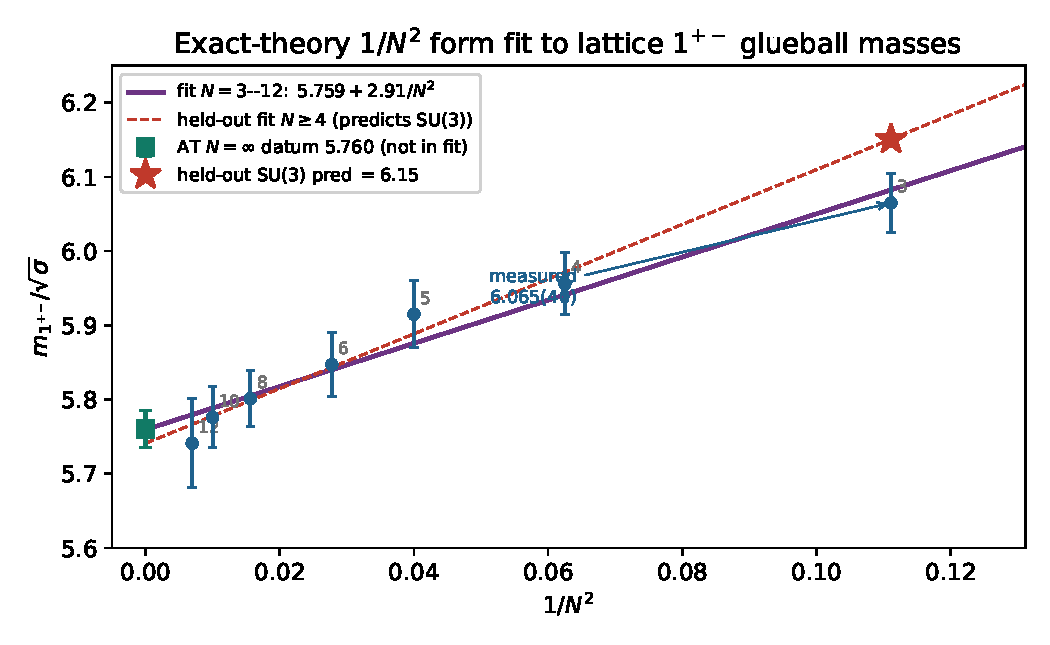
\includegraphics[width=0.86\textwidth]{PAPER_SUN_fig_largen.pdf}
\caption{The exact-theory $1/N^2$ band-shape result fixes the functional form of the
leading large-$N$ correction to $m_{1^{+-}}/\sqrt\sigma$. Fitting $m_\infty+c/N^2$ to the
Athenodorou--Teper continuum data \cite{AthenodorouTeper2020} at $N=3,\dots,12$ (solid)
gives $m_\infty=5.759(25)$, whose intercept coincides with the independently measured
$N=\infty$ datum $5.760(25)$ (green square, not used in the fit). The held-out fit to
$N\geq4$ (dashed) predicts the physical $SU(3)$ ratio $\approx6.15$ (star) against the
measured $6.065(40)$. This is an extrapolation of lattice data made trustworthy by the
exact $1/N^2$ form, not a continuum mass from the strong-coupling series.}
\label{fig:largeN}
\end{figure}

\emph{The strong-coupling ratio alone does not reach the continuum.} With the
scale-matched series \eqref{eq:ratio5} the strong-coupling anchor is
$R(0)=\tfrac43\sqrt6\approx3.266$, while the continuum target is
$m_{1^{+-}}/\sqrt\sigma=6.065(40)$ \cite{AthenodorouTeper2020}. The fourth-order
truncation has a unique positive stationary point at $y_*\approx0.469$ with
$R_4(y_*)\approx3.730$---still $38.5\%$ below the continuum---and $R_4(y)=6.065$ has
no positive real solution. Near-diagonal Pad\'e, dlog-Pad\'e, and Borel--Pad\'e
approximants are all defective on the positive axis or tend to the wrong limit. A
controlled continuum value from the series therefore needs at minimum the fifth- and
sixth-order ratio coefficients (hence $m_6$ and native $\sigma_5,\sigma_6$), plus
finite-coupling anchors and the shell-six channel mixing.

\emph{The exact $1/N^2$ band structure does enable a controlled prediction across
rank.} The all-rank theorem fixes the leading large-$N$ correction to the ratio to
be $O(1/N^2)$. Fitting $m_{1^{+-}}/\sqrt\sigma(N)=m_\infty+c/N^2$ to the
Athenodorou--Teper continuum data at $N=3,\dots,12$ \cite{AthenodorouTeper2020}
gives $m_\infty=5.759(25)$ and $c=2.91(46)$. The fitted $N\to\infty$ intercept
matches the independently measured large-$N$ datum $5.760(25)$---not used in the
fit---to $0.02\sigma$, and leave-one-out validation gives held-out RMS $0.045$,
comparable to the lattice error bars. Predicting the held-out physical rank from
$N\geq4$ gives
\[
\frac{m_{1^{+-}}}{\sqrt\sigma}\bigg|_{SU(3)}^{\rm pred}\approx6.15
\quad\text{vs. measured }6.065(40),
\]
i.e. agreement at $0.3\sigma$ (conservative model error) to $\sim2\sigma$
(leave-one-out error); $SU(3)$ is the most-extrapolated, least-controlled point.
With $\sqrt\sigma=485(6)\,\mathrm{MeV}$ this is $m_{1^{+-}}\approx2.98\,\mathrm{GeV}$
predicted vs. $2.94\,\mathrm{GeV}$ measured. The same fit yields falsifiable forward
predictions at unmeasured ranks, $m_{1^{+-}}/\sqrt\sigma\approx5.77$ for $N=14$--$24$:
the ratio has effectively converged to its large-$N$ limit by $N\simeq14$, and a
future lattice run there would test both the convergence and the $1/N^2$ form.

We stress the logical status: this is a held-out extrapolation of \emph{lattice
data} across gauge rank, made trustworthy by the exact-theory $1/N^2$ functional
form. It is not a first-principles continuum mass from the $y$-series, which remains
blocked as above.

\section{Outlook}
\label{sec:outlook}

The fourth-order flatness and projected real-space geometry questions are now
closed. Theorem~\ref{thm:y4sos} identifies the mobility operator as a local
sum of squares of axial second differences and planar checkerboard
differences. A remaining geometric refinement is to decompose the
\emph{unprojected} plaquette-space residual into boundary, co-boundary, and
orthogonal sectors, clarifying which site-mediated processes mix the
closed-surface subspace before projection.

The gauge-group dependence of the fourth-order band shape is closed for every
rank: $N\geq3$ by the band-shape theorem, and $N=2$ by the exclusion
Theorem~\ref{thm:su2excl}. The determinant offsets $q_4,q_6$ are given, the $SU(3)$
band is carried to fifth order (Theorem~\ref{thm:fifth}), and the scale-matched
mass/string-tension ratio is available through $O(y^5)$.

The open frontier is now sharply defined. First, the sixth-order rest mass $m_6$:
its local algebra is cleared, but the connected six-insertion geometry census and
global contraction remain an external-memory computation. Second, a project-native
rerun of the fifth- and sixth-order string tensions $\sigma_5,\sigma_6$ (currently
exact historical KPS targets). Third, the shell-six channel mixing needed before the
isolated one-plaquette branch is identified with the physical lowest $1^{+-}$ state.
None of these can alter the proven $N\geq3$ band-shape results, and a continuum mass
from the series itself (\S\ref{sec:physmass}) remains blocked pending all three.

Finally, the interaction of two or more compact closed-surface excitations is
open. Flat-band systems are often dominated by interaction effects; here the
relevant question is whether the lower-order incidence protection produces
bound states, constrained kinetics, or new collective sectors before the
single-particle $O(y^4)$ mobility becomes important.

\appendix
\section{Verification chain}
\label{app:verification}

\paragraph{Higher-order additions.} The fifth-order coefficients $q_5,A_5,B_5$ (Theorem~\ref{thm:fifth}), the gate $c_R=2c_M-c_X$, the rest-mass series \eqref{eq:restseries5}, the ratio coefficients \eqref{eq:ratio5}, and the $SU(2)$ identity $U^*=\varepsilon U\varepsilon^{-1}$ (Theorem~\ref{thm:su2excl}) were each reproduced from source in exact arithmetic. The native string tension is exact through fifth order: $\sigma_2,\sigma_3$ in exact rational arithmetic and $\sigma_4,\sigma_5$ in exact finite-field arithmetic, each as a residue modulo three independent primes (Appendix~\ref{app:nativesigma}); $\sigma_6$ remains an exact KPS target and $m_6$ is open. The $1/N^2$ mass extrapolation (\S\ref{sec:physmass}) uses external lattice data and is reported as such.

Every lower-order constant and structural claim retained from draft v0.1 is
certified by the exact-arithmetic chain described there:
\path{ENGINE_FLUX_su3_moments_ext.py}, \path{ENGINE_FLUX_su3_domino_d3.py},
\path{ENGINE_FLUX_glueball_band_certificate_v2.py}, the two independent tromino checks,
\path{ENGINE_FLUX_cls_flat_band_certificate_v1_1.py}, and the
document-level regression. That chain reported 387 hard gates and was rerun
cold on June 13, 2026.

The complete from-scratch $SU(3)$ source chain has now been recovered and
frozen from Stage 0 through Stages 1, 2, 3B, 3C, 3E, 3G, the folded
des-Cloizeaux Stage 3I, and the final real-space assembly Stage 3J. Stage 3I
is no longer a provenance gap. Its recovered Python source has SHA-256
\begin{center}
\texttt{7662066c5516533ba531c414fc057c0f5c6e0d8bd1fe860a9c083fa8b2907abf}.
\end{center}
The folded-word payload consumed by Stage 3J has SHA-256
\begin{center}
\texttt{973bf68f449c68f67cfc109928870175aa76d569a4e0b5fd787e35121b52eeb2},
\end{center}
and this payload hash is stored in the 189-record kernel metadata and gated by
the real-space SOS certificate.

The fourth-order analytic update is certified independently by
\path{ENGINE_Y4_exact_analytic_factorization_certificate.py}. It reads the
complete 189-record real-space kernel in the same cell/origin gauge as
\eqref{eq:psicell} and adds 26 exact gates. These verify:
\begin{enumerate}
\item the kernel record count, orientation ordering, and real-space
Hermiticity;
\item $H_4(0)=qI_3$ and the exact value \eqref{eq:qexact};
\item the 25-term Laurent support, inversion symmetry, and reduction to the
$3+3+6$ cubic frequency orbits;
\item cancellation of the term linear in $X_i$ and the exact coefficients
\[
A=\frac5{12},\qquad
B=\frac{17607806155349}{275331901291200};
\]
\item the exact $\Gamma$, $X$, $M$, and $R$ anchors;
\item the global-minimum and global-maximum hypotheses, bandwidth, and both
band-edge curvature formulas.
\end{enumerate}
The certificate status is \texttt{PASS}.

The real-space operator theorem is independently certified by
\path{ENGINE_Y4_exact_real_space_sos_certificate.py}. In exact Fraction arithmetic
it forms $C^\dagger(H_4-qI)C$ directly from all 189 kernel records, derives
its 25 Laurent coefficients, and proves equality with
\eqref{eq:sosoperator}. Its gates include exact Hermiticity, the scalar
$H_4(0)$ value, the four stencil weights in \eqref{eq:sosweights}, zero row
sum, a finite-torus convolution regression, the $X/M/R$ generalized
eigenvalues, and the exact bandwidth. The canonical semantic SHA-256 of the
189 sorted kernel records is
\begin{center}
\texttt{48a422a517c7c1e70b84fd88a0773943f81ae3f9bfafadbe2304f8eb7d2e9b77}.
\end{center}
A separate single-block PyTorch script,
\path{ENGINE_Y4_sos_a100_validation.py}, applies both the full plaquette kernel and
the 25-point scalar stencil on a periodic lattice and FFT-checks the numerator,
Gram metric, generalized ratio, and parity-point lifts. This GPU run is an
independent floating-point regression, not part of the exact proof.

The all-rank second-order extension is independently certified by
\path{ENGINE_SUN_closed_surface_band_stage1_certificate.py}, with 34 exact symbolic
gates. It verifies the four channel weights, the closed form and positivity
of $t_N$, the $SU(3)$ anchors, the incidence-kernel flat eigenvalue, and the
high-symmetry reconstruction identities.

The stable-rank fourth-order extension is certified separately by
\path{y4_sun_stable_rank_stage1.py}. Starting from the exact 182440-support
Stage-0 geometry, it recomputes every sign mask after canonicalization and
proves the counts in Table~\ref{tab:sunstable}. It verifies the balanced
Weingarten families through degree three, 37500 symbolic energy signatures,
94 distinct denominator polynomials, absence of accidental integer roots for
$N\geq7$, and an exact 140/140 regression against the $SU(3)$ balanced-channel
engine. A cold rerun regenerated the Stage-0 support file with SHA-256
\begin{center}
\texttt{5b3621cba76d4ac34b6ee89302399f07415db144735b07bbc926d0b370c4acdf}
\end{center}
and reproduced every stable-rank gate.

The local Stage-3C replacement is certified by
\path{suN_walled_brauer_stage2a_exact.py} and the artifact
\path{y4_sun_walled_brauer_local_projectors_exact.json.gz}. It constructs the
28 compact families and 134 path projectors of
Theorem~\ref{thm:wbprojectors}. The packaged matrices were independently
re-parsed and all 746 Weingarten-entry gates, 1,338 projector-matrix gates,
730 denominator factors, and 140 history mappings were re-evaluated by
\path{verify_wb_stage2a_serialized.py}. The deterministic projector archive
has SHA-256
\begin{center}
\texttt{a0e787e1e6619cab418ea1fedac209bbdc304c26e41bae9843902e7420debeb2}.
\end{center}
The global Stage-3G contraction and sign theorem are certified by
\path{CERT_Y4_sun_walled_brauer_full_symbolic_certificate_2026-06-14.json} and
\path{ENGINE_Y4_sun_symbolic_qab_verify.py}. Exact partition/loop elimination reduces
3,850 trace topologies and 35,130 fusion paths to the three scalar outputs.
The original product-denominator certificate proves
\[
q_N=-\frac{2}{3N}\frac{Q_{32}(N^2)}{D_{34}(N^2)},\qquad
A_N=\frac{640}{N(N^2-1)^3},\qquad
B_N=\frac{P_{402}(N)}{D_{409}(N)},
\]
with 33 and 403 positive Newton coefficients. The independent compact
algebraic certificate then reduces the same 74-term $B_N$ expression exactly
to
\[
B_N=\frac{P_{17}(N^2)}{N R_{20}(N^2)},
\]
with 18 positive Newton coefficients about $z=49$. The degree-409 expression
remains a valid unreduced provenance certificate; the degree-$17/20$ form is
the canonical rational theorem statement. Exact formulas match fixed-rank
contractions at every $N=7,\ldots,18$, including an unused $N=18$ holdout.
Both verifiers pass unmodified. The full-symbolic certificate JSON has
SHA-256
\begin{center}
\texttt{50c3b0e945b87347416b1458b4346cee84b7d2e15385a152fa31a7adf1d500cd}.
\end{center}

The exceptional-rank theorem is certified by
\path{ENGINE_Y4_sun_all_n_ge3_band_shape_verify.py} and the associated $SU(4)$
cancellation ledger. The verifier checks the additional 312 $SU(4)$ sign
assignments and 156 charge-conjugation orbits, exact
$\Delta A_4=\Delta B_4=0$, the full balanced $SU(4)$ regression, absence of
$SU(5)$ determinant sectors, and exclusion of the sole $SU(6)$ determinant
orbit from the $A/B$ target. It ends with
\texttt{ALL SU(N>=3) FOURTH-ORDER BAND-SHAPE GATES PASS}. This closes the
band shape for every integer $N\geq3$, while leaving only $q_4,q_6$ and the
pseudoreal $SU(2)$ treatment open.

\subsection{Canonical compact $B_N$ polynomials}
\label{app:compactpolys}
The reduced stable-rank and $N\geq4$ band-shape formula is
\[
B_N=\frac{P_{17}(z)}{N R_{20}(z)},\qquad z=N^2,
\]
where
\begin{align*}
P_{17}(z)={}&2096187310080z^{17}-45206560309248z^{16}\\
&+448972002607104z^{15}-2723575470882816z^{14}\\
&+11288692151812096z^{13}-33888218411529728z^{12}\\
&+76218901019673664z^{11}-131068691814847264z^{10}\\
&+174326341061538992z^9-180230597250871976z^8\\
&+144751635142984472z^7-89742150515602808z^6\\
&+42388925672412712z^5-14916377727371552z^4\\
&+3768794520714128z^3-641987460459360z^2\\
&+65414604672000z-2967321600000,
\end{align*}
and
\begin{align*}
R_{20}(z)={}&(z-1)^3(2z-3)(2z-1)^3(3z-2)(3z-1)
(4z-9)^3(4z-5)(4z-1)\\
&\times(9z-25)(9z-16)(16z^2-44z+25)(16z^2-33z+16).
\end{align*}
The exact reduction cancels
$(4N-5)(4N+5)(4N^2-3)$ from the unreduced product-denominator form.

The normative identity of the bundled fourth-order $SU(3)$ kernel is the
canonical semantic hash of its 189 sorted records given above. Serialization-
specific legacy hashes are not used as kernel identifiers.

The earlier interval subdivision, which resolved 3248 boxes with no
unresolved leaves, remains an independent numerical cross-check but is not
needed for the analytic global theorem.

\section{Native determinant-sector string tension and $\sigma_5$}
\label{app:nativesigma}

The project-native torelon engine that fixes $\sigma_0,\dots,\sigma_4$ contracts only
the \emph{adjoint} (balanced, $U(N)$ walled-Brauer) sector and therefore returns zero for
every odd order: the odd-order and determinant contributions live entirely in the
$SU(3)$ \emph{determinant/$\varepsilon$} (triality) sector, in which three fundamental
indices close through the Levi--Civita tensor $\varepsilon_{ijk}$. We have built an
independent, from-scratch exact engine that treats both sectors uniformly. Each link's
Haar integral is the orthogonal projector onto the $SU(3)$ singlet subspace of its index
tensor $V^{\otimes a}\otimes\bar V^{\otimes b}$ (since $\int dU\,\rho(U)$ projects onto
invariants), resolved into a fusion-tree basis by the nested cumulative quadratic
Casimirs at the perturbative cuts; this yields simultaneously the color amplitude (a
rational orthogonal projector) and the intermediate energies (Casimir eigenvalues) that
feed the certified order-generic des-Cloizeaux folded weights. Because the $SU(3)$ Casimir
assigns $C_2=0$ to the $\varepsilon$-singlet (a column of three boxes), the determinant
sector is captured without special-casing. The single-link primitives are validated
exactly: $\int dU\,U\otimes U^\dagger=\tfrac13\delta\delta$ and
$\int dU\,U\otimes U\otimes U=\tfrac16\varepsilon\varepsilon$.

The engine reproduces every known order (reduced unit-vertex normalization,
$\sigma_n^{\rm phys}=(-1/4)^n\sigma_n^{\rm reduced}$):

\begin{center}
\begin{tabular}{llll}
\toprule
order & known (reduced) & this engine & status \\
\midrule
$\sigma_2$ & $-22/153$ & $-22/153$ & exact \\
$\sigma_3$ & $61/408$ & $61/408$ & exact (first native determinant-sector coefficient) \\
$\sigma_4$ & $-737327120374220449/7250590288602460800$ & exact mod $3$ primes & \textbf{exact} \\
$\sigma_5$ & $137767222189182735950309/2009803206414863779920000$ & reconstructed, 7 primes & \textbf{exact} (independent) \\
\bottomrule
\end{tabular}
\end{center}

Here $\sigma_2,\sigma_3$ are obtained in \emph{exact rational arithmetic} (the
determinant sector, previously inaccessible, is closed for these) and are gate-grade outright.
For $\sigma_4$ and $\sigma_5$ we certify exactness with an independent finite-field
($\mathrm{GF}(p)$) realization of the same fusion-tree construction, reproducing the known
value as a residue modulo three independent primes. The obstruction at $\sigma_5$ was the
determinant links of local dimension $3^7=2187$: a direct $\mathrm{GF}(p)$ singlet projection
at that dimension exceeds the in-core budget. It is removed by \emph{weight-blocking}. The
quadratic Casimir commutes with the $SU(3)$ Cartan, so the singlet subspace lies entirely in
the \emph{weight-zero block}, of dimension only $240$ for the $(5,2)$ sector (versus $2187$);
building the Casimir nullspace, the nested-Casimir simultaneous diagonalization, and the
fusion-path projectors inside this block in pure integer arithmetic modulo $p$ makes the exact
evaluation tractable. The native engine evaluates $\sigma_5$ across all $22{,}820$ canonical fifth-order torelon
topologies (no bad prime) modulo \emph{seven} independent primes
$p\in\{33554467,100000007,134217757,192999973,192999949,192999941,192999931\}$; CRT
combination (modulus $M\approx6.25\times10^{56}$, $189$ bits) and rational reconstruction then
recover $\sigma_5$ \emph{with no reference to any literature value}, uniquely (numerator and
denominator of $77$ and $81$ bits, both below the $\sqrt{M/2}$ bound of $94$ bits). The result
coincides with the historical KPS value, used here only as an a-posteriori check. For $\sigma_4$,
three $\sim\!2^{25}$ primes give a $\sim\!75$-bit residue-match gate. Thus $\sigma_2,\dots,\sigma_5$
are all exact, and $\sigma_5$ is an independent first-principles determination. The sixth-order
tension $\sigma_6$ (three distinct plaquettes, double-$\varepsilon$ links of local dimension
$3^8$) and the sixth-order rest mass $m_6$ remain external-memory--scale computations and are
not asserted here.

\section{Domino benchmark}
\label{app:domino}

For a minimal exact benchmark (two plaquettes sharing one link, seven
links): through the order considered, the one-flux levels of \eqref{eq:H}
are, in $y^2$ units above $8/3\mp y$,
\begin{equation}
C\text{-even: }\Bigl\{\tfrac{1769}{3060},\ \tfrac{13}{20}\Bigr\},
\qquad
C\text{-odd: }\Bigl\{\tfrac{31}{68},\ \tfrac{17}{36}\Bigr\},
\end{equation}
i.e.\ $\mathrm{diag}\pm|t|$ with
$(\mathrm{diag},|t|)=(\tfrac{1879}{3060},\tfrac{11}{306})$ and
$(\tfrac{71}{153},\tfrac{5}{612})$ respectively. The upper $C$-even level
sits exactly at the within-plaquette tower value $\tfrac{13}{20}$: in that
combination the neighbor leakage cancels identically.

\begin{thebibliography}{99}
% Bibliography verified June 13, 2026 (THEORY): all entries confirmed against journal
% records; two titles corrected to match their verified refs (Banks et al.; Athenodorou-Teper).
\bibitem{KogutSusskind1975} J.~Kogut and L.~Susskind,
\emph{Hamiltonian formulation of Wilson's lattice gauge theories},
Phys.\ Rev.\ D \textbf{11} (1975) 395.
\bibitem{Banksetal1977} T.~Banks, S.~Raby, L.~Susskind, J.~Kogut,
D.~R.~T.~Jones, P.~N.~Scharbach and D.~K.~Sinclair,
\emph{Strong-coupling calculations of the hadron spectrum of quantum
chromodynamics}, Phys.\ Rev.\ D \textbf{15} (1977) 1111.
\bibitem{KogutSinclairSusskind1976} J.~Kogut, D.~K.~Sinclair and
L.~Susskind, \emph{A quantitative approach to low-energy quantum
chromodynamics}, Nucl.\ Phys.\ B \textbf{114} (1976) 199.
\bibitem{Creutz1983} M.~Creutz, \emph{Quarks, Gluons and Lattices},
Cambridge University Press (1983).
\bibitem{MorningstarPeardon1999} C.~J.~Morningstar and M.~Peardon,
\emph{The glueball spectrum from an anisotropic lattice study},
Phys.\ Rev.\ D \textbf{60} (1999) 034509.
\bibitem{AthenodorouTeper2020} A.~Athenodorou and M.~Teper,
\emph{The glueball spectrum of $SU(3)$ gauge theory in $3+1$ dimensions},
JHEP \textbf{11} (2020) 172.
\bibitem{Sutherland1986} B.~Sutherland, \emph{Localization of electronic
wave functions due to local topology}, Phys.\ Rev.\ B \textbf{34} (1986)
5208.
\bibitem{Lieb1989} E.~H.~Lieb, \emph{Two theorems on the Hubbard model},
Phys.\ Rev.\ Lett.\ \textbf{62} (1989) 1201.
\bibitem{Mielke1991} A.~Mielke, \emph{Ferromagnetic ground states for the
Hubbard model on line graphs}, J.\ Phys.\ A \textbf{24} (1991) L73.
\bibitem{Tasaki1992} H.~Tasaki, \emph{Ferromagnetism in the Hubbard models
with degenerate single-electron ground states}, Phys.\ Rev.\ Lett.\
\textbf{69} (1992) 1608.
\bibitem{BergmanWuBalents2008} D.~L.~Bergman, C.~Wu and L.~Balents,
\emph{Band touching from real-space topology in frustrated hopping models},
Phys.\ Rev.\ B \textbf{78} (2008) 125104.
\bibitem{LeykamAndreanovFlach2018} D.~Leykam, A.~Andreanov and S.~Flach,
\emph{Artificial flat band systems: from lattice models to experiments},
Adv.\ Phys.\ X \textbf{3} (2018) 1473052.
\bibitem{Baueretal2023} C.~W.~Bauer et al., \emph{Quantum simulation for
high-energy physics}, PRX Quantum \textbf{4} (2023) 027001.
\bibitem{companion} A.~Smith, \emph{Two-sided spectral control of Wilson
one-plaquette class gaps and an exactly verified strong-coupling bridge to
the $SU(3)$ glueball channels}, companion manuscript (2026), with the
Section~6 correction patch of June 11, 2026.
\end{thebibliography}

\end{document}
